%%%%%%   TIPO DE DOCUMEN%TO: Reporte   %%%%%%
\documentclass[letterpaper,11pt]{report}
%%%%%%%%%%%%%%%%%%%%%%%%%%%%%%%%%%%%%%%%%%%%

%%%%%%%   PAQUETES   %%%%%%%
\usepackage[spanish]{babel}
\usepackage{graphicx}
\usepackage[utf8]{inputenc}
%\usepackage[latin1]{inputenc}
\usepackage{float}
\usepackage{multirow}
\usepackage{amsmath}
\usepackage{amssymb}
\usepackage{eurosym} 
\usepackage{longtable}
\usepackage{colortbl}
%%%%%%%%%%%%%%%%%%%%%%%%%%%%

%%%%%%%%%%%%%%%%%%%%%%%%%%%%%%%%%%%%%%%%
%%%%%%%   INICIO DEL DOCUMENTO   %%%%%%%
%%%%%%%%%%%%%%%%%%%%%%%%%%%%%%%%%%%%%%%%
\begin{document}

    %%%%%%% Renombrar en espaNol %%%%%%
    \renewcommand{\tablename}{Tabla} %Escribe Tabla en lugar de Cuadro
    \renewcommand{\listtablename}{\'Indice de tablas} %Escribe Indeice de tablas en lugar de Indice de cuadros

    %%%%%%%   PORTADA   y RESUMEN   %%%%%%% Este es el contenido agregado de la secci\'on 2.

    %%%%%%%%%%%%%%%%%%%%%%%%%%%%%
%%%%%      PORTADA      %%%%%
%%%%%%%%%%%%%%%%%%%%%%%%%%%%%

\begin{titlepage}

    \centering %Todo centrado

    %%%%  LOGO DE LA ESCUELA   %%%%
    
\includegraphics[scale=0.17]{imagenes/escom-ipn} %Imagen para portada
    %%%%  NOMBRE DE LA ESCUELA   %%%%
    \LARGE{\\ Instituto Polit\'ecnico Nacional}
    \LARGE{\\ Escuela Superior de C\'omputo}
    
    \vspace{1cm} %Espacio vertical

    %%%%  TITULO Y NÚMERO DE TRABAJO   %%%%
    \LARGE \textbf{ Nombre del Trabajo Terminal}
    \LARGE {\\ Número de Trabajo Terminal}

    \vspace{1cm} %Espacio vertical

    \LARGE \textit{Que para cumplir con la opción de titulación curricular en la carrera de:}
    \LARGE \textbf{\\ Ingeniería en Sistemas Computacionales}

    \vspace{1cm} %Espacio vertical

    %%%%   ALUMNOS   %%%%
   \textit{Presentan}\\
    Alumno 1 \\
    Alumno 2 \\
    Alumno 3

    \vspace{1cm} %Espacio vertical

    %%%%   Directores   %%%%
   \textit{Directores}\\
    M. en C. José David Ortega Pacheco \bigskip  Director 2

\end{titlepage} %incluye el archivo portada.tex
    %%%%%%%%%%%%%%%%%%%%%%%
%%%%    RESUMEN    %%%%
%%%%%%%%%%%%%%%%%%%%%%%

\begin{abstract}

  Aquí va el resumen general del documento de trabajo terminal.

\end{abstract}
 %Incluir resumen del documento (resumen.tex)
	%%%%%%%%%%%%%%%%%%%%%%%
%%%%  ADVERTENCIA  %%%%
%%%%%%%%%%%%%%%%%%%%%%%

\begin{small}
	
	\centering \textbf{Advertencia} 
	
\end{small}


	\textit{“Este documento contiene información desarrollada por la Escuela
		Superior de Cómputo del Instituto Politécnico Nacional, a partir de datos y
		documentos con derecho de propiedad y por lo tanto, su uso quedará
		restringido a las aplicaciones que explícitamente se convengan.”} \\
	
		La aplicación no convenida exime a la escuela su responsabilidad técnica y
		da lugar a las consecuencias legales que para tal efecto se determinen. \\
		
		Información adicional sobre este reporte técnico podrá obtenerse en: \\
		
		La Subdirección Académica de la Escuela Superior de Cómputo del Instituto
		Politécnico Nacional, situada en Av. Juan de Dios Bátiz s/n Teléfono:
		57296000, extensión 52000.
		






		 %Incluir advertencia del archivo (advertencia.tex)
	%%%%%%%%%%%%%%%%%%%%%%%
%%% AGRADECIMIENTOS %%%
%%%%%%%%%%%%%%%%%%%%%%%

\large{\textbf{Agradecimientos}} \\

Gracias a Dios por la vida de mis padres y mi hermano, por ser los principales promotores de mis sueños, gracias a ellos por cada día confiar y creer en mí y mis expectativas, gracias a la vida por este nuevo triunfo, gracias a todas las personas que me apoyaron y creyeron en la realización de este proyecto. \\
Intenta hasta el final, y no te detengas ante la duda; Nada es tan difícil, la búsqueda lo demostrará. \textbf{Robert Herrick
} \\

\begin{flushright}
	\textbf{Tanya Silvana Hernández Valdez} 
\end{flushright} 

Gracias a mis padres: María de la Luz Correa y José Luis Chávez por apoyarme y quererme
siempre en cada día de desvelo por estudio, trabajo y dedicación; a mis hermanos: Marisol
Chávez y José Iván Chávez por aguantar mis días estresados llenos de trabajo y cansancio,
siguiendo el ejemplo de mis padres siempre apoyándome y queriéndome día con día; a mi
novio Luis Antonio Dávila por estar a mi lado apoyándome todos y cada uno de los días de
escuela, impulsándome con cada palabra de aliento y amándome día con día en los momentos
fáciles y difíciles siendo mi inspiración completa; y por ultimo a mis directores: María del
Rosario Rocha y Juan Carlos Morales por transmitirnos sus conocimientos, aportándonos
ideas en este proyecto.\\

\begin{flushright}
	\textbf{Diana Ivonne Chávez Correa} \\
\end{flushright} 
 %Incluir agradecimientos del archivo (agradecimientos.tex)
    %%%%%%%   INCLUIR ENCABEZADOS EN INDICES Y CAPITULOS   %%%%%%%
    \pagestyle{headings}

    %%%%%%%   NUMERACION EN CONTENIDO E INDICE DE TABLAS Y FIGURAS   %%%%%%%
    \pagenumbering{roman} %NUmeros romanos
    %\setcounter{page}{1} %Comienza en I por default, aquI se puedo modificar

    %%%%%%   INCLUIR CONTENIDO, INDICE DE FIGURAS E INDICE DE TABLAS   %%%%%%
    \tableofcontents
    \listoffigures
    \listoftables

    %%%%%%%   NUMERACION EN CAPITULOS   %%%%%%%
    \clearpage %Para iniciar con los arAbigos
    \pagenumbering{arabic} %Numeros arabigos
    %\setcounter{page}{1} %Comienza en 1 por default, aquI se puede modificar

    %%%%%%%   INCLUYE CAPITULOS Y SECCIONES   %%%%%%%
    \chapter{Introducci\'on}

La Clasificación Internacional del Funcionamiento de la Discapacidad y de la Salud (CIF) define la discapacidad como un término genérico que engloba deficiencias, limitaciones de actividad y restricciones para la participación social. La discapacidad forma parte de la condición humana: “… casi todas las personas sufrirán algún tipo de discapacidad transitoria o permanente en algún momento de su vida, y las que lleguen a la senilidad experimentarán dificultades crecientes de funcionamiento”. \\

De acuerdo a los informes de la Organización Mundial de la Salud (OMS), se estima que más de mil millones de personas viven con algún tipo de discapacidad; es decir, alrededor del 15\% de la población mundial (según las estimaciones de la población mundial en 2010) \cite{uno}. En relación con lo anterior, en el país existen 31.5 millones de hogares, de ellos 6.1 millones reportan que existe al menos una persona con discapacidad; es decir, en 19 de cada 100 hogares vive una persona que presenta alguna dificultad. \\

En el 2013 6.6\% de la población mexicana reportó tener una discapacidad, siendo en su mayoría las personas adultos mayores, con 51.4\%, informó el Instituto Nacional de Estadística y Geografía (INEGI). Por otra parte, la Encuesta Nacional de Ingresos y Gastos de los Hogares 2012 (ENIGH 2012), dicho porcentaje de la población del país presentó dificultad (discapacidad) para realizar al menos una de las actividades como: caminar, ver, escuchar, hablar o comunicarse, poner atención o aprender, atender el cuidado personal y mental \cite{dos}. Mientras que en los adultos mayores la enfermedad y la edad es el factor detonante. En los adultos mayores, el 50.9\% de las discapacidades se tienen por origen de la edad avanzada. \\
De acuerdo con las proyecciones del Consejo Nacional de Población (CONAPO), hasta 2010 la población en el Distrito Federal de 65 años en adelante representa el 7.9\% del total. Para 2030, serán los “viejitos” del futuro y demandarán productos y servicios especiales para ellos. \\

Aunado a este factor, "las Instituciones del Gobierno y la oferta de salud entre hospitales y personal especializado no son suficientes para atender a la población que sufre de alguna discapacidad, por otra parte del costo por estos servicios es elevado oscilando desde \$7,000 M.N. a \$30,000 M.N. mensuales \cite{tres}. \\

En la actualidad existen programas sociales por parte del Gobierno de la Ciudad de México, uno de ellos es “Médico en tu casa” este programa fue creado para reducir índices de mortalidad por embarazos en Iztapalapa y Gustavo A. Madero. El cual consiste en enviar médicos para que atiendan a mujeres embarazadas, adultos mayores y niños. El principal objetivo de este programa es brindar atención a la población vulnerable, principalmente adultos mayores, discapacitados, enfermos terminales, así como disminuir el índice de mortalidad materna-infantil en la capital. \\

Sumado a lo anterior es necesario utilizar herramientas que nos permitan facilitar el cuidado de las personas con discapacidad, dando una opción más accesible para la población que no cuente con recursos necesarios para pagar algún servicio de cuidado y atención. \\

La idea de utilizar este tipo de herramientas es facilitar el cuidado y la atención de las personas con alguna discapacidad, teniendo en cuenta que aún pueden realizar actividades de la vida cotidiana, además de estar pendientes de los momentos exactos en los que la persona presente una situación delicada en su estado de salud. Una de estas alternativas es utilizar sensores que permitan supervisar las vulnerabilidades que presente, buscando aprovechar al máximo el tiempo de los familiares sin descuidar la atención que requiere el familiar con discapacidad, sin dejar de lado la necesidad de reducir los precios que conlleva el cuidado de las personas con discapacidad, ya que con esta propuesta permitirá a los familiares que no cuenten con los recursos para este tipo de servicios, puedan usarla como apoyo al cuidado de sus familiares, siendo el costo del prototipo más accesible, pensando en que se realice con un menor monto al requerido por las instituciones que brindan estos servicios. \\




	   \section{Contexto de trabajo}

Se describe el área donde se esta trabajando y en qué contexto
	   \section{Problemática}

   
	   \section{Trabajo previo}

  
	   \section{Justificación}

Como se mencionó anteriormente la discapacidad en el país ha ido en aumento en los últimos años debido a la transición demográfica, la reducción de mortalidad-natalidad y accidentes ocasionados en el trabajo. La mayor parte de la población discapacitada son los adultos mayores de 60 años. Es decir, la enfermedad o la edad avanzada son las principales causas para todos los tipos de discapacidad considerados. Con el desarrollo de este prototipo se pretende dar atención a una necesidad social que cada vez va en aumento, debido a los altos costos que implica contratar un servicio especializado que aún no se encuentra plenamente desarrollado. Aunque es necesario puntualizar que este prototipo solo supervisará aquellos casos en los que el adulto mayor no se encuentre postrado en una cama. \\


\begin{table}[htb]
	\centering
	\begin{tabular}{|p{4cm}|p{1.5cm}|p{1.5cm}|p{1.5cm}|p{1.5cm}|}
		\hline
		Tipos de discapacidad & \multicolumn{4}{c|}{Grupos de edad} \\
		\cline{2-5} 
		& 0 a 14 años & 15 a 29 años & 30 a 59 años & 60 años o más \\
		\hline \hline
		Caminar, subir o bajar usando sus piernas. & 36.2 & 32.1 & 56.2 & 81.3 \\ \cline{2-5}
		\hline 
		Ver (aunque usen lentes). & 26.9 & 44.6	& 58.2 & 67.2 \\ \cline{2-5}
		\hline 
		Mover o usar sus brazos o manos. & 14.1 & 18.2 & 28.5 &	42.7 \\ \cline{2-5}
		\hline 
		Aprender, recordar o concentrarse. & 40.8 & 31.5 & 32.1 & 44.6 \\ \cline{2-5}
		\hline 
		Escuchar (aunque usen aparato auditivo). & 13.4	& 18.5 & 24.2 & 46.9 \\ \cline{2-5}
		\hline 
		Bañarse, vestirse o comer. & 37.4 & 16.4 & 14.5 & 29.3 \\ \cline{2-5}
		\hline 
		Hablar o comunicarse. & 45.6 & 28.5 & 13.4 & 14.0 \\ \cline{2-5}
		\hline 
		Problemas emocionales o mentales. & 26.6 & 28.0 & 20.1 & 16.3  \\ \cline{2-5}
		\hline
	\end{tabular}
	\textbf{\caption{\small{\textbf{Porcentaje de población con discapacidad, por tipo de discapacidad según grupos de edad en 2014 \cite{diez}.}}}}
	\label{Justificacion:Tabla1.1}
\end{table}

Por lo que se requiere de servicios especializados en salud enfocados a este sector, en la actualidad existen programas para atender este tipo de problemáticas por mencionar algunos provenientes del Gobierno de la Ciudad de México como: 

\begin{itemize}
	\item Médico en tu casa.
	\item Programa Nacional para el Desarrollo y la Inclusión de las personas con discapacidad.
\end{itemize}

Por parte de la iniciativa Privada existen servicios para este tipo de necesidad como:

\begin{itemize}
	\item Cuidado personalizado (Homewatch Care Givers).
	\item Estancia (La Casa de Las Lunas).
\end{itemize}

Teniendo costos elevados que desequilibran la economía familiar, tal y como se mencionó en la introducción de la investigación. Sin embargo, los programas gubernamentales no logran cubrir la demanda para estos servicios y por parte de la iniciativa privada sus costos son elevados, como consecuencia no toda la población cuenta con los recursos suficientes para pagar un servicio como esté. \\
 
Por lo que se propone un prototipo para ayudar a personas con determinada discapacidad, implementando una serie de alertas que permitan a los familiares estar al tanto de la situación del discapacitado, por otro lado, se busca que este prototipo sea portable y económico, de esta manera reducir los costos que significa este tipo de cuidados, siendo una alternativa o complemento de los servicios ya existentes. \\

Para cubrir la necesidad de la población con bajos recursos, se piensa diseñar una tarjeta de propósito específico a partir de sensores y microcontroladores adecuados con el fin de reducir los costos, ya que estos son muy accesibles en el mercado, utilizados para múltiples aplicaciones permitiendo que el prototipo sea escalable y portable. \\

Entre las diferencias con respecto a lo ya existente, son las alertas instantáneas emitidas por los sensores logrando mantener al familiar informado de la situación en la que se encuentra la persona con discapacidad. Cabe mencionar que los sistemas de monitoreo existentes están diseñados para que una persona esté siempre monitoreando la situación del discapacitado.


 
	   \section{Marco Teórico}

A continuación se presentan las variables que consideramos importantes para el desarrollo del proyecto, antes de llevar a cabo la elección de los dispositivos a emplear, previamente se elaboró una investigación de los signos vitales más indispensables del ser humano, por lo que para fines del proyecto y de acuerdo con lo analizado las variables a medir son la temperatura, considerando que es el primer parámetro para determinar una enfermedad, la segunda variable es un acelerómetro que por causa del envejecimiento de las personas suelen ser más predispuestas a sufrir alguna caída y por último la frecuencia cardíaca, esta última involucra un órgano muy importante para las personas por ello consideramos evaluar conjuntamente esta medida. Existen otras variables importantes pero por la complejidad para medirlas no entran en la posibilidad de incluirlas en este trabajo terminal, dichas variables pueden ser por ejemplo: la presión arterial, la glucosa, por mencionar algunas, ya que al medirlas no utilizan un método invasivo y no causan molestia al usuario. 

\subsection{Variables a medir}

En este apartado se muestra una descripción de las variables que elegimos y la importancia de cada una, de igual forma se explicaran los motivos por los que fueron seleccionadas. A continuación se en listan las variables seleccionadas y las cuales serán monitoreadas en este proyecto:

\begin{enumerate}
	\item Temperatura.
	\item Caídas.
	\item Frecuencia Cardíaca.
\end{enumerate}

\begin{enumerate}
	\item \textbf{Temperatura} 
	
	Se ha considero medir la temperatura corporal, está variable es de gran importancia para determinar las condiciones en las que se encuentra el enfermo, la constante medición de esta permite a enfermeros(as) y algún otro personal médico conocer la mejoría y situación del paciente, en algunos casos la temperatura se toma como primer parámetro para diagnosticar una enfermedad. \\
	
	La Secretaria de Salud establece que la temperatura corporal aceptable oscila entre los $36.5^{\circ}$C $47^{\circ}$C y los $37.2^{\circ}$C, mientras que las temperaturas fuera de este rango se consideran anormales, a continuación, se muestran los términos utilizados considerados anormales conforme a la Norma Oficial Mexicana NOM-031-SSA2-1999, considerando que no interviene un mecanismo termorregulador o se presenta un golpe de calor.
	
	\begin{itemize}
		\item \textbf{Fiebre:} La elevación anormal de la temperatura corporal por encima de los $38^{\circ}$C.
		\item \textbf{Hipertermia:} Es el estado de incremento de la temperatura del cuerpo que sobrepasa los $40^{\circ}$C.
		\item \textbf{Hipotermia:} En este estado la temperatura corporal se encuentra por debajo de los $36^{\circ}$C.
	\end{itemize}
	
	Por esta razón es importante tener controlada la temperatura en el rango que se considera aceptable. Nuestro cuerpo tiene mecanismos que regulan la temperatura y con el paso de los años se van perdiendo. Por esta importancia se decidió tomar la temperatura como una de las variables a medir en este proyecto \cite{once}.
	
	\item \textbf{Caídas}
	
	Las caídas son consideradas de alta importancia, debido las consecuencias que conllevan y pueden sufrir las personas de la tercera edad. Los tipos de caídas en adultos mayores pueden ser las siguientes:
	
	\begin{itemize}
		\item \textbf{Caída accidental:} Es aquella que generalmente se produce por una causa ajena al adulto mayor sano (ejemplo: tropiezo) y que no vuelve a repetirse.
		\item \textbf{Caída repetida:} Expresa la persistencia de factores predisponentes como, enfermedades crónicas múltiples, fármacos, pérdidas sensoriales, etc.
		\item \textbf{Caída prolongada:} Es aquella en la que el adulto mayor permanece en el suelo por más de 15 o 20 minutos por incapacidad de levantarse sin ayuda.	Los adultos mayores que tienen mayor prevalencia de caídas prolongadas son: aquellos de 80 años o más, con debilidad de miembros, con dificultades para las actividades cotidianas y aquellos que toman medicación \cite{doce}.
	\end{itemize}

	\begin{itemize}
		\item Escenarios y posturas de una persona al sufrir una caída.
		Para entender los escenarios y posturas se realizó un estudio con 240 personas de la tercera edad para monitorear sus actividades cotidianas (como: sentarse en una silla, sentarse en un inodoro, salir o entrar de un auto, sentarse o recostarse sobre la cama y caminar), a estas personas se les coloca un acelerómetro en diferentes partes del cuerpo, el cual detecta las señales tanto de las actividades mencionadas, como de alguna caída (caídas hacia delante o atrás, caídas laterales a la izquierda o derecha y caídas con las piernas rectas o flexionadas) que lleguen a sufrir los sujetos de estudio \cite{trece}. \\
		 
		En la figura 1.3 se detectaron los umbrales superior e inferior de caídas, donde se observa que estas tienen una señal con un pico muy alargado el cual está en un rango de aceleración de entre 0 y 7 g, a diferencia de la señal de las actividades cotidianas que no rebasan 1.5 g. \\
		
		\begin{figure}[h]
			\centering
			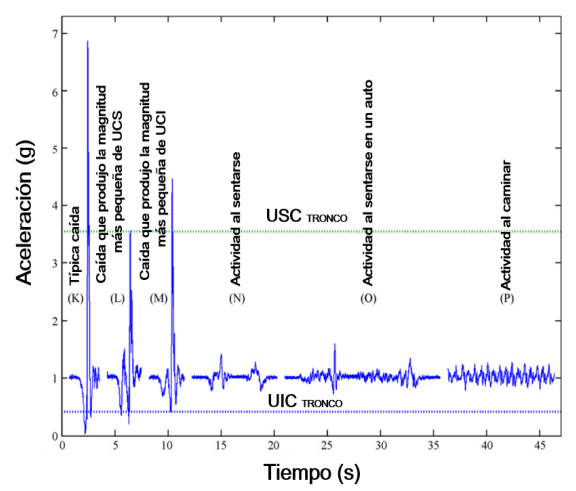
\includegraphics[scale=0.35]{introduccion/imagenes/grafica1_3}
			\textbf{\caption{\small{Representación de una señal para caídas y actividades cotidianas, en personas de la tercera edad usando un acelerómetro \cite{trece}.}}}
			\label{Seccion1.5.1:Figura1.3}
		\end{figure}
		
		En la figura 1.4 se muestran detalladamente los puntos de interés en la señal y cada una de las posiciones en las que se encontraba el adulto mayor al sufrir una caída, de igual manera se muestran detalladamente las actividades cotidianas realizadas en donde el acelerómetro registro actividad con pequeñas variaciones y similitudes, mostrando los puntos de interés en dicha señal.  \\
		
		\begin{figure}[h]
			\centering
			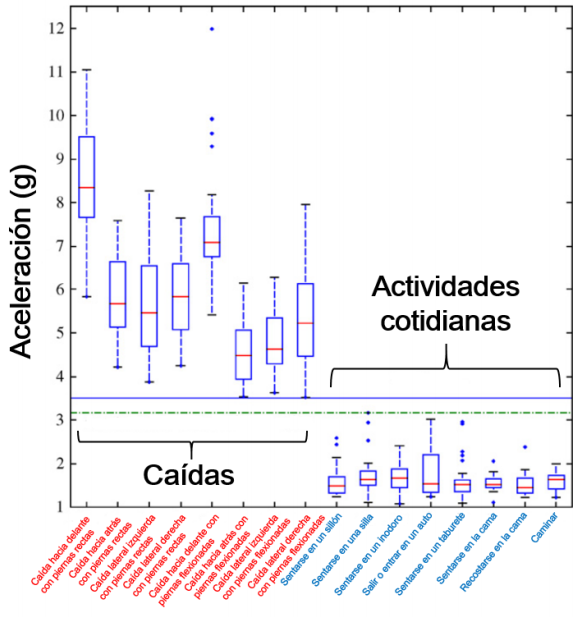
\includegraphics[scale=0.35]{introduccion/imagenes/grafica1_4}
			\textbf{\caption{\small{Puntos de interés en la señal que muestra: (a) posturas al sufrir una caída y (b) actividades cotidianas \cite{trece}.}}}
			\label{Seccion1.5.1:Figura1.4}
		\end{figure}
		
		Con base en las figuras 1.3 y 1.4 se establecen los escenarios en los que una persona puede sufrir algún tipo de caída y en donde se utilizan sensores acelerómetros en diferentes partes del cuerpo para realizar un muestreo de la aceleración. \\
		
		\begin{table}
%			\centering
			\resizebox*{12.5cm}{8cm}{
				\begin{tabular}{|l|c|c|c|}
					\hline
					Escenario & Postura	& Muestreo del acelerómetro & Caída \\
					\hline \hline
					Caída hacia adelante con piernas rectas	& De pie o recostado & 7.5g a 9.5g & Si \\
					\hline
					Caída hacia atrás con piernas rectas & De pie o recostado & 5g a 6.5g & Si \\
					\hline
					Caída lateral izquierda con piernas rectas & De pie o recostado & 4.5g a 6.5g & Si \\
					\hline
					Caída lateral derecha con piernas rectas & De pie o recostado & 5g a 6.5g & Si \\
					\hline
					Caída hacia adelante con piernas flexionadas & Sentado o inclinado & 6.8g a 7.8g & Si \\
					\hline
					Caída hacia atrás con piernas flexionadas & Sentado o inclinado & 4g a 5g & Si \\
					\hline
					Caída lateral izquierda con piernas flexionadas & Sentado o inclinado & 4.5g a 5.5g & Si \\
					\hline
					Caída lateral derecha con piernas flexionadas & Sentado o inclinado & 4.8g a 6g	& Si \\
					\hline
					Sentarse en un sillón & Sentado	& 1.2g a 1.8g & No \\
					\hline
					Sentarse en una silla & Sentado & 1.5g a 1.9g &	No \\
					\hline
					Sentarse en un inodoro & Sentado & 1.5g a 2g & No \\
					\hline
					Salir o entrar de un auto & Sentado o de pie & 1.2g a 2.5g & No \\
					\hline
					Sentarse en un taburete & Sentado & 1.2g a 1.5g & No \\
					\hline
					Sentarse en la cama	& Sentado & 1.4g a 1.6g & No \\
					\hline
					Recostarse en la cama & Recostado & 1.2g a 1.6g & No \\
					\hline
					Caminar & De pie & 1.5g a 1.8 & No \\
					\hline
				\end{tabular}
			}
		\textbf{\caption{\small{\textbf{Escenarios y posturas en los que el acelerómetro realizará muestreo.}}}}
		\end{table}
	
	 Por lo anterior y debido a la complejidad de detectar todos los escenarios de caídas, en este proyecto únicamente se detectará la caída típica, que es la caída hacia delante con las piernas rectas.
	\end{itemize}

	\item \textbf{Frecuencia Cardíaca}
	
	Esta variable es considerada importante puesto que involucra uno de los signos más relevantes para el óptimo funcionamiento del corazón, de modo que es el principal órgano del ser humano que nos mantiene con vida, por lo cual estimaremos dicha variable para este proyecto. \\
	
	El funcionamiento del corazón se manifiesta, al actuar como bomba impulsora, lo que determina el gasto cardíaco (cantidad de sangre enviada por el corazón al torrente circulatorio en un minuto), que representa el volumen de eyección sistólico en cada latido por minuto. La frecuencia cardíaca (FC) es un parámetro indicativo de la eficiencia con la que el corazón trabaja. En esfuerzos de tipo máximo se busca alcanzar la frecuencia cardíaca máxima para cada sujeto, sin pasar los límites que representen riesgo de provocar una falla o insuficiencia cardíaca durante la ejecución de un esfuerzo físico intenso. Para determinarla existen varios modelos matemáticos, pero el más común consiste en tomar la cifra de 220 y restarle la edad del sujeto. \\
	
	Por otro lado, habitualmente la tensión arterial se incrementa con la edad, más la sistólica que la diastólica, así como la presión del pulso (diferencia entre ambas), en las personas mayores de 65 años, el 40\% sufre de hipertensión arterial, y de ellos el 65\% - 70\% tienen riesgo de sufrir accidentes cardiovasculares, fatales o no. \\
	
	Con el paso de los años, el organismo pierde su habilidad para redistribuir el flujo sanguíneo desde las vísceras a los músculos en acción, de tal forma que la diferencia arteriovenosa de oxígeno (Dif a/v O2) medida en el músculo y la del flujo de retorno venoso al corazón durante el esfuerzo físico, es menor en las personas adultas mayores y sedentarias, con lo cual disminuye la reserva funcional \cite{catorce}. \\
	
	Algunos estudios realizados en poblaciones sanas, así como en pacientes hipertensos, con cardiopatía isquémica o con insuficiencia cardíaca, demuestran una asociación entre la FC elevada y un mayor riesgo de mortalidad. Según esto, cuanto mayor es la FC, menor es la expectativa de vida. La frecuencia cardíaca (FC) en reposo oscila entre 50 y 100 latidos por minuto en las personas adultas. Al nacer, la FC es más elevada porque el bebé la necesita para su adecuado crecimiento. A partir del primer mes de vida, la FC va disminuyendo hasta alcanzar las cifras normales de un adulto. El ejercicio físico o las situaciones de estrés provocan un aumento de la FC (taquicardia sinusal), que se considera normal \cite{quince}.
	
\end{enumerate}

\subsection{Sensores}

A continuación, se muestran algunas definiciones de la investigación de los sensores que ayudaran a la realización de este proyecto. \\

Un dispositivo electrónico que produce datos eléctricos, ópticos o digitales derivadas de una condición física o evento. La Real Academia Española lo define como un dispositivo que detecta una determinada acción externa y es transmitida adecuadamente. \\

Conociendo estas definiciones llamaremos sensor al dispositivo o mecanismo eléctrico que nos permite medir una variable física, dando como respuesta una señal o dato en relación con la magnitud de la variable medida. 

\subsection{Sensor de temperatura}

\textbf{Definición} \\

Es un dispositivo que permite medir los cambios de la temperatura y entregar una señal eléctrica en relación a la magnitud de la temperatura. Son usados para asegurar que la temperatura de un proceso esté en su normalidad o bien tener la temperatura en un rango especificado siendo obligatorio cumplir con la condición. \\

La variedad de sensores de temperatura está relacionada con el material del que están hechos, del uso que se les pretenda dar en función con las temperaturas que soporten y como es que responden a la magnitud medida, estas respuestas pueden ser en voltaje, resistencia, corriente y señales digitales. \\

Entre los más utilizados se encuentran los termistores NTC (Coeficiente de Temperatura Negativa) y PTC (coeficiente de temperatura Positiva), termopares, RTD (Detectores de Temperatura por Resistencia), circuitos integrados y detectores de temperatura por luz infrarroja. \\


\begin{figure}[h]
	\centering
	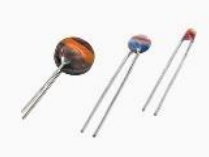
\includegraphics[scale=0.35]{introduccion/imagenes/termistores}
	\textbf{\caption{\small{Termistores \cite{dieciseis}.}}}
	\label{Seccion1.5.1:Figura1.5}
\end{figure}

\textbf{Tipos de sensores de temperatura} \\

\textbf{RTD} \\

Los RTD son sensores de temperatura que utilizan la propiedad de resistencia y coeficiente térmico de un metal (conductor), se basan en el principio de equilibrio térmico que señala que cuando un metal se encuentra en un medio que tiene mayor temperatura que él, éste tiende a aumentar su temperatura, siempre y cuando el volumen y la masa no sean mayor que el del medio con el que interactúa. Las RTD son utilizadas en el sector industrial, entre las características más destacadas es su resistencia a altas temperaturas, su alta sensibilidad, tienen una exactitud mínima de $1^{\circ}$C, tienen un tiempo de vida alto. \\

\textbf{NTC} \\

Las NTC son sensores elaborados por óxidos semiconductores que responden disminuyendo su resistencia a medida que aumenta la temperatura, son sensores con alta sensibilidad, son utilizados para monitorear que la temperatura no sobrepase un rango. \\

\textbf{PTC} \\

Las PTC son termistores con un coeficiente de temperatura positivo que al aumentar la temperatura aumenta su resistencia, son elaborados con óxidos y conductores, se utilizan para elaborar sistemas de control de temperatura, con el fin de no sobrepasar cierta temperatura ya que esta puede ser critica \cite{diecisiete}. \\

\textbf{Termopares} \\

Son sensores que se elaboran uniendo dos conductores, están basados en el principio de Seebeck y Peltier, el efecto de Seebeck dice que cuando la unión de los metales presenta diferentes temperaturas se produce un voltaje muy pequeño, que va en incremento con la temperatura, mientras que el efecto Peltier dice que transmitir una corriente en la unión de los metales se produce un flujo de calor. Los termopares se utilizan en sistemas de refrigeración para disminuir las temperaturas o aumentarlas, además de sensar la temperatura \cite{dieciocho}. \\

\textbf{Sensores a base de Circuitos Integrados} \\

Los circuitos integrados son dispositivos que están formados de elementos electrónicos, que permiten tener la misma funcionalidad que un circuito electrónico, solo que en un espacio reducido. En la actualidad tienen funciones específicas desde reguladores de voltaje, corriente hasta medir temperatura. \\

\textbf{Sensores Infrarrojos} \\

Otra de las propuestas interesantes que tenemos son los sensores de radiación térmica, estos funcionan midiendo la energía que emiten los objetos, en la región infrarroja, están construidos por un sistema óptico que enfoca el objeto, utilizando un diodo láser que ilumina la zona captando la energía desprendida de los objetos. \\

Presentan un inconveniente acorde a los materiales que presentan emisividad, que es la proporción de radiación térmica emitida por una superficie u objeto debido a su temperatura. \\

Los cuerpos negros presentan una emisividad igual a uno, en la práctica todos los cuerpos tienen esta propiedad de acuerdo a su color, los sensores de radiación vienen ajustados para una emisividad predeterminada, por lo que si se tiene otra emisividad diferente se tendrá que calibrar \cite{diecinueve}. 

\subsection{Sensor acelerómetro}
\renewcommand{\theequation}{\arabic{equation}}
\newcounter{neq}
\setcounter{equation}{\arabic{neq}}

\textbf{Definición} \\

Como ya se mencionó anteriormente, los acelerómetros son dispositivos que miden la aceleración, que es la tasa de cambio de la velocidad de un objeto y son útiles para detectar las vibraciones en los sistemas o para aplicaciones de orientación \cite{veinte}. \\

El acelerómetro calcula la aceleración por medio de la siguiente formula: \\

\begin{equation}
	\alpha = \frac{F}{m}
	\addtocounter{neq}{1}
\end{equation} \\

Dicha fórmula es la segunda ley de Newton y establece que, en un cuerpo con masa constante, la aceleración del cuerpo es proporcional a la fuerza que actúa sobre él mismo, dónde $\alpha$ es la aceleración, \textit{F} es la fuerza y \textit{m} la masa de un cuerpo. \\

La aceleración se calcula en unidades de metro por segundo al cuadrado (m/s2), o en fuerza G (g), que es aproximadamente de 9.8 m/s2. Los acelerómetros son dispositivos electromecánicos que detectan las fuerzas de aceleración, ya sea estática (incluyen gravedad) o dinámica (incluyen vibraciones y movimiento) \cite{veinte}. \\

El giroscopio se basa en el efecto Coriolis para medir la velocidad angular, el cual consiste en una masa de prueba de resonancia montada en el silicio. El giroscopio es, a diferencia de un acelerómetro, un sensor activo. La masa de prueba es empujada hacia atrás y hacia adelante por peines de conducción. Una rotación del giroscopio genera una fuerza de Coriolis que actúa sobre la masa que se traduce en un movimiento en una dirección diferente. El movimiento en esta dirección se mide mediante electrodos y representa la velocidad de giro \cite{veintiuno}. \\

El giroscopio calcula la velocidad angular por medio de la siguiente formula: \\

\begin{equation}
	\varPhi = \frac{d\theta}{dt}
	\addtocounter{neq}{1}
\end{equation} \\

Dicha fórmula establece que, la velocidad angular es la tasa de cambio del desplazamiento angular por unidad de tiempo, es decir que tan rápido gira un cuerpo alrededor de su eje y las unidades de velocidad angular son radianes por segundo (rad/s). \\

\textbf{Tipos de sensores acelerómetros \cite{veintidos}:} \\ 

\begin{itemize}
	\item \textbf{Acelerómetros mecánicos} \\
	
	Acelerómetros mecánicos, tales como el acelerómetro de masa sísmica, el sensor de velocidad, y el interruptor magnético mecánico, detectan la fuerza impuesta sobre una masa cuando se produce aceleración. La masa se resiste a la fuerza de la aceleración y de este modo provoca una deformación o un desplazamiento físico, que puede ser medido por los detectores de proximidad o galgas extensiométricas (como se muestra a continuación). Muchos de estos sensores están equipados con dispositivos de amortiguación, tales como muelles o imanes para impedir la oscilación. 
	
	\begin{figure}[h]
		\centering
		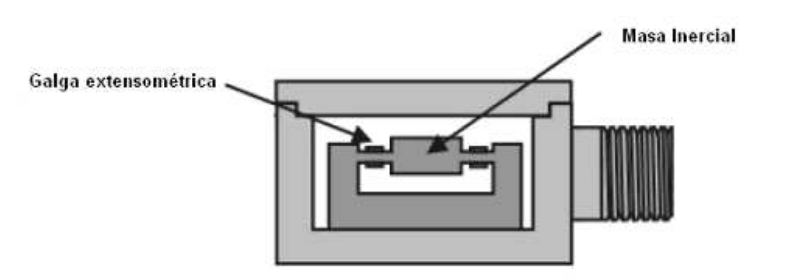
\includegraphics[scale=0.35]{introduccion/imagenes/acelerometro_mecanico}
		\textbf{\caption{\small{Acelerómetro tipo mecánico \cite{veintitres}.}}}
		\label{Seccion1.5.4:Figura1.6}
	\end{figure}

	\item \textbf{Acelerómetros Piezoeléctricos} \\
	
	Acelerómetros piezoeléctricos son ampliamente utilizados para la aceleración de propósito general, mediciones de choque y vibración. Básicamente son transductores de movimiento con grandes señales de salida y comparativamente de pequeños tamaños. Están disponibles con muy altas frecuencias naturales y son por lo tanto adecuados para aplicaciones de alta frecuencia y mediciones de choque. Estos dispositivos utilizan una masa en contacto directo con el componente piezoeléctrico, o cristal. Cuando un movimiento variable se aplica al acelerómetro, el cristal experimenta una excitación de fuerza variable, causando una carga proporcional q eléctrica a ser desarrollada a través de esta. Se clasifican en dos tipos: \\
	
	\begin{enumerate}
		\item El primero de ellos es el acelerómetro de salida de carga de alta impedancia. En este tipo de acelerómetro, el cristal piezoeléctrico genera una carga eléctrica que está conectada directamente a los instrumentos de medición. La salida de carga requiere instalaciones e instrumentación especiales, que habitualmente encontramos en los centros de investigación. Este tipo de acelerómetro también se emplea en aplicaciones de altas temperaturas $(>120^{\circ}C)$ en las que no se pueden utilizar modelos de baja impedancia. \\
		
		\item El segundo tipo de acelerómetro es el acelerómetro de salida de baja impedancia. Un acelerómetro de baja impedancia incluye un acelerómetro de carga en su extremo delantero, así como un minúsculo microcircuito integrado y un transistor FET (de efecto de campo) que convierte la carga en una tensión de baja impedancia que puede interaccionar fácilmente con la instrumentación estándar. Este tipo de acelerómetro es el que se emplea habitualmente en la industria. Una fuente de alimentación para acelerómetro como la ACC-PS1 proporciona al microcircuito un suministro eléctrico adecuado de 18 a 24 V a una corriente constante de 2 mA y elimina la corriente de polarización CC. Este tipo de fuente de alimentación suele generar una señal de salida a partir de cero de hasta +/- 5 V dependiendo del índice mV/g del acelerómetro. 
		
		\begin{figure}[h]
			\centering
			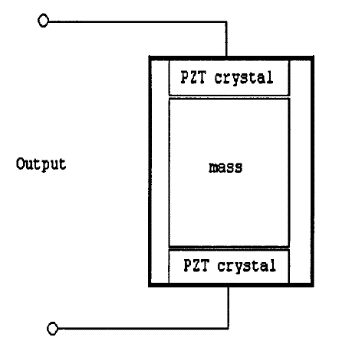
\includegraphics[scale=0.55]{introduccion/imagenes/acelerometro_piezoelectrico}
			\textbf{\caption{\small{Acelerómetro tipo piezoeléctrico \cite{veintitres}.}}}
			\label{Seccion1.5.4:Figura1.7}
		\end{figure}		
	\end{enumerate}

	\item \textbf{Acelerómetros Piezoresistivos} \\
	
	Acelerómetros piezoresistivos son esencialmente medidores de deformación de semiconductor con grandes factores de calibre factores de alto calibre se obtienen debido a que la resistividad del material depende principalmente de la tensión, no sólo en las dimensiones. El aumento de la sensibilidad es crítica en la medición de la vibración, ya que permite la miniaturización del acelerómetro. La mayoría de los acelerómetros piezorresistivos utilizan dos o cuatro calibradores activos dispuestos en un puente de Wheatstone. Se utilizan resistencias extra de precisión, como parte del circuito en serie con la entrada para controlar la sensibilidad, equilibrio y la compensación de los efectos de temperatura. En algunas aplicaciones, topes de sobrecarga son necesarios para proteger los medidores de insumos de alta amplitud. Estos instrumentos son útiles para la adquisición de información de vibración a bajas frecuencias (por ejemplo, por debajo de 1 Hz). De hecho, los sensores piezorresistivos son inherentemente verdaderos dispositivos de medición de aceleración estática. Las características típicas de acelerómetros piezorresistivos pueden ser 100 mV g-1 en la sensibilidad, 0 - 750 Hz en rango de frecuencia, 2500 Hz en la frecuencia de resonancia, 25 g en rango de amplitud, 2,000 g en índice de choque, de 0 a 95$^{\circ}$C en el rango de temperatura, con una masa total de aproximadamente 25g. Los sensores piezoresistivos operan con elementos extensométricos son sensibles a la temperatura y requieren una compensación. Se prefieren para las aplicaciones de vibraciones de baja frecuencia, descarga de larga duración, y de aceleración constante. Las unidades piezoresistivas son resistentes, y pueden operar a frecuencias de hasta 2,000 Hz. 
	
	\begin{figure}[h]
		\centering
		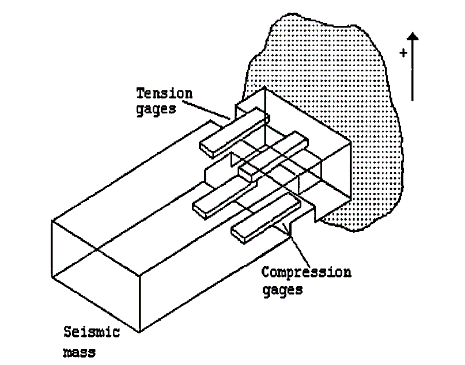
\includegraphics[scale=0.55]{introduccion/imagenes/acelerometro_piezoresistivo}
		\textbf{\caption{\small{Acelerómetro tipo piezoresistivo  \cite{veintitres}.}}}
		\label{Seccion1.5.4:Figura1.8}
	\end{figure} 

	\item \textbf{Acelerómetros capacitivos} \\
	
	Acelerómetros diferencial-capacitancia se basan en el principio del cambio de la capacitancia en proporción a la aceleración aplicada. Vienen en diferentes formas y tamaños. En un tipo, la masa sísmica del acelerómetro se hace como el elemento móvil de un oscilador. La masa sísmica se apoya en una disposición de haz paralelo de movimiento elástico de la base. El sistema se caracteriza por tener una cierta frecuencia nominal definida cuando no alterados. Si se acelera el instrumento, la frecuencia varía por encima y por debajo del valor nominal, dependiendo de la dirección de la aceleración. En acelerómetros de capacidad de detección, micro mecanizados de placas capacitivas (placas de condensador CMOS solo 60 micras de profundidad) forman una masa de unos 50 micro gramos. Como la aceleración deforma las placas, un cambio de capacitancia es medible. \\
	
	\begin{figure}[h]
		\centering
		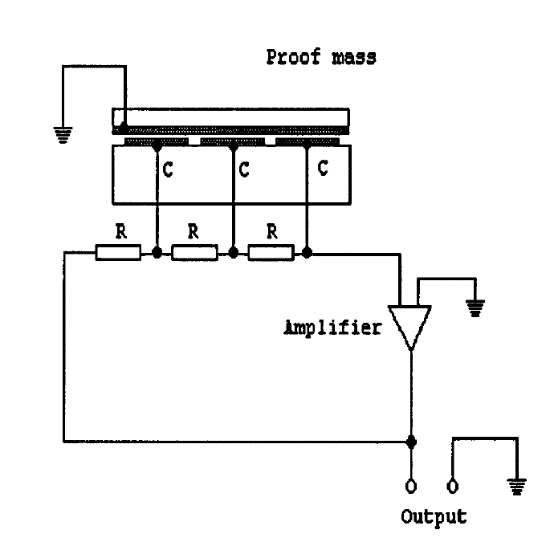
\includegraphics[scale=0.55]{introduccion/imagenes/acelerometro_capacitivo}
		\textbf{\caption{\small{Acelerómetro de capacitivo \cite{veintitres}.}}}
		\label{Seccion1.5.4:Figura1.9}
	\end{figure} 

	\item \textbf{Acelerómetro térmico} \\
	
	Estos acelerómetros hacen uso de una masa sísmica que está suspendida por un resorte o una palanca dentro de un marco rígido. El marco que lleva la masa sísmica está conectado firmemente a la fuente de vibración que tenga características medibles. Como el sistema vibra, la masa tiende a permanecer fija en su posición de modo que el movimiento puede ser registrado como un desplazamiento relativo entre la masa y el marco. Este desplazamiento es detectado por un transductor apropiado y la señal de salida se procesa adicionalmente. Sin embargo, la masa sísmica no permanece absolutamente constante; pero para frecuencias seleccionadas, de manera satisfactoria puede actuar como una posición de referencia. Mediante la selección apropiada de la masa, la primera, y combinaciones de los amortiguadores, los instrumentos sísmicos pueden ser utilizados ya sea para la aceleración o mediciones de desplazamiento. En general, una gran masa y resorte suave son apropiados para mediciones de vibración y de desplazamiento, mientras que una masa relativamente pequeña y resorte rígido se utilizan en acelerómetros. Este sensor detecta la posición a través de la transferencia de calor. Una masa sísmica se coloca encima de una fuente de calor. Si la masa se mueve a causa de la aceleración, la proximidad de la fuente de calor y la temperatura de la masa cambia. Las termopilas de polisilicio se utilizan para detectar cambios en la temperatura. 
	
	\begin{figure}[h]
		\centering
		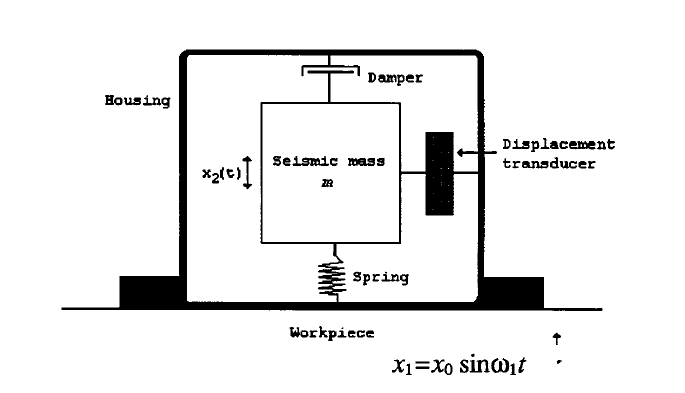
\includegraphics[scale=0.55]{introduccion/imagenes/acelerometro_termico}
		\textbf{\caption{\small{Acelerómetro térmico \cite{veintitres}.}}}
		\label{Seccion1.5.4:Figura1.10}
	\end{figure} 

	\item \textbf{Acelerómetro con tecnología MEMS} \\
	
	Estos acelerómetros son ampliamente utilizados en aplicaciones como: dinámica de vehículos, detección de orientación de teléfonos móviles, estabilidad de imagen, inclinación, detección de golpes y dispositivos antirrobo. \\
	
	Los acelerómetros de capacitancia variable están disponibles en varias configuraciones, incluidos sensores de vibraciones basados en un circuito oscilador sintonizable y sistemas mecánicos micro eléctricos (MEMS). Los circuitos de oscilador sintonizable incorporan un capacitor con una placa que actúa como una masa móvil tipo diafragma en relación con otras placas fijas. La aceleración hace que el diafragma se flexione, creando un cambio capacitivo. Esto cambia la tensión pico de la oscilación. Los acelerómetros MEM se implementan como un capacitor variable modificado por una viga en voladizo conectada a una masa de prueba. Están disponibles en dispositivos compatibles con 1 a 3 ejes. Acelerómetros MEMS utilizan interfaces seriales como I2C y SPI. Tienen alta linealidad y se utilizan mayormente en aplicaciones de baja frecuencia. 
	
	\begin{figure}[h]
		\centering
		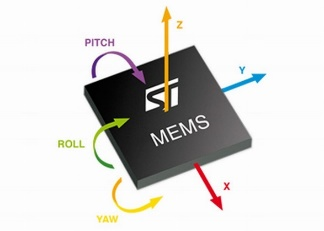
\includegraphics[scale=0.75]{introduccion/imagenes/acelerometro_MEMS}
		\textbf{\caption{\small{Acelerómetro con tecnología MEMS \cite{veinticuatro}.}}}
		\label{Seccion1.5.4:Figura1.11}
	\end{figure} 
\end{itemize}

\subsection{Sensor de frecuencia cardíaca}

\textbf{Definición} \\

La frecuencia cardíaca permite medir la cantidad de sangre por minuto que llega al corazón, por ello para determinar esa variable necesitamos un dispositivo que mida la frecuencia del corazón, por lo tanto a continuación se dará una definición del sensor para este tipo de variable, es un dispositivo conformado por un transmisor y un receptor conformados por fotodiodos, los cuales tienen la función de detectar la cantidad de sangre que fluye dependiendo de la zona donde sea colocado en un determinado tiempo. \\

\textbf{Tipos de sensores de frecuencia cardíaca} \\ 

\textbf{Óptico} \\

Emplean fotocélulas como elementos de detección. A veces disponen de un cabezal que contiene un emisor de luz y la fotocélula de detección del haz reflejado sobre el objeto. Otros trabajan en modo barrera y se utilizan para cubrir mayores distancias, con fuentes luminosas independientes del detector. Ambos tipos suelen trabajar con frecuencias en la banda de infrarrojos. Su utilización principal es como detectores de posición. El principio de funcionamiento está basado en la generación de un haz luminoso por parte de un fotoemisor, que se proyecta sobre un fotorreceptor, o bien, sobre un dispositivo reflectante. La interrupción o reflexión del haz, por parte del objeto a detectar, provoca el cambio de estado en la salida de la fotocélula. \\

Se clasifican según su sistema de detección: 

\begin{itemize}
	\item Sistema de detección de “barrera”
	\item Sistema de detección “réflex” 
	\item Sistema de detección “autoreflex”	
\end{itemize}

\textbf{Fotoeléctrico de barrera} \\

Dispone de emisor y receptor de haz luminoso dispuestos separadamente. \\

\textbf{Óptico tipo réflex} \\

Concentra en un solo bloque el emisor y receptor, siendo más fácil su instalación, aunque requiere un dispositivo reflector. Para este cometido se suele emplear un sistema catadióptrico, que tiene la propiedad del triedro trirectangular, el cual refleja la luz en la misma dirección en la que llega. Dispone de una mayor distancia de detección que el sistema de barrera, teniendo en cuenta que el trayecto que recorre el haz de luz es el doble. \\

\textbf{Óptico tipo autoreflex} \\

En este sistema es el propio objeto a detectar el que funciona como elemento reflector, lo cual simplifica la tarea de instalación. Por el contrario, su inconveniente es que dispone de una menor distancia de detección en comparación con los dos tipos anteriores. Las ventajas de este tipo de detectores son la inmunidad a perturbaciones electromagnéticas, las grandes distancias de detección, alta velocidad de respuesta, identificación de colores y detección de pequeños objetos. Una variable importante son los construidos de fibra óptica que permite separar el punto emisor y el detector de la unidad principal del sensor con las ventajas de accesibilidad que ello proporciona \cite{veinticinco}. \\

\textbf{Tecnología fotopletismografía} \\

La fotopletismografía está basada en la medida y análisis de una señal óptica relacionada con los cambios en el volumen sanguíneo, que permite medir la componente pulsátil del latido del corazón y evaluar así la circulación sanguínea Esta técnica es ampliamente usada en la práctica médica como parte de los pulsioxímetros, para medir el pulso, equivalente al ritmo cardíaco, y la saturación de oxígeno, o relación entre la concentración de hemoglobina oxigenada y la concentración total de hemoglobina, habitualmente en la punta de los dedos \cite{veintiseis}. \\

\textbf{Principios Físicos:} Detecta el flujo de sangre cutáneo y traduce sus pulsaciones. Consiste en la emisión de luz infrarroja desde un diodo emisor y un fotodetector adyacente que recibe la luz infrarroja reflejada. A medida que aumenta el flujo de sangre cutáneo aumenta la cantidad de luz reflejada. De esta manera obtenemos una medida cualitativa del flujo sanguíneo cutáneo. Se utiliza preferentemente en la medición de la presión digital. \\

\textbf{Oxímetros} \\

La oximetría de pulso es un método no invasivo que permite la estimación de la saturación de oxígeno de la hemoglobina arterial y también vigila la frecuencia cardiaca y la amplitud del pulso \cite{veintisiete}. \\

Para la determinación de la saturación de hemoglobina arterial con oxígeno (SpO2), el oxímetro de pulso o pulsioxímetro usa la espectrofotometría basada en que la oxihemoglobina u hemoglobina oxigenada (HbO2) y la desoxihemoglobina o hemoglobina reducida (Hb) absorben y transmiten determinadas longitudes de onda del espectro luminoso para la luz roja (640-660nm) y la luz infrarroja (910-940nm). La HbO2 absorbe más la luz infrarroja y permite el paso de la luz roja; por el contrario, la Hb absorbe más la luz roja (R) y permite el paso de la luz infrarroja (IR). El radio de la absorción de la luz R e IR mide el grado de oxigenación de la hemoglobina. \\

Los oxímetros de pulso tienen dos sensores o sondas con diodos emisores de luz (LED), uno para luz IR y otro para la R, además, de un fotodiodo detector. Para medir el oxígeno los LED y el fotodiodo detector deben ponerse en puntos opuestos dejando en medio el tejido translucido (pulpejo del dedo, pabellón auricular, etc). El mecanismo que permite la lectura de la oxigenación es que en cada pulsación de la sangre arterial se transmiten valores lumínicos, detectando al mismo tiempo la frecuencia cardíaca \cite{veintiocho}. 

\subsection{Microcontroladores}

En la actualidad el uso de microcontroladores es indispensable para desarrollar aplicaciones dedicadas, debido a que contienen una variedad de módulos que nos permiten interactuar con el mundo físico en tiempo real. A continuación, definiremos los conceptos teóricos que utilizaremos en la elaboración del proyecto, dando una noción de la utilidad que nos aporta un microcontrolador. Antes de mencionar a los microcontroladores es necesario mencionar que es un microprocesador ya que es su antecesor. \\

El microprocesador es un circuito integrado que contiene solo la unidad central de procesamiento (CPU), es utilizado para procesar grandes volúmenes de información, para ser utilizados es necesario conectar dispositivos periféricos.
En el siguiente apartado tenemos algunas definiciones de microcontrolador. \\

Es un circuito integrado o chip que incluye en su interior las tres unidades funcionales de un computador: CPU, memoria y unidades de entrada y salida, pero con capacidades limitadas y un alto nivel de especialización. \\

Lo definimos como un dispositivo dedicado, que en su memoria sólo reside un programa destinado que permite controlar una aplicación determinada, sus unidades de entrada y salida soportan la conexión de sensores y dispositivos de control que permitan efectuar el proceso deseado. Es un microprocesador optimizado, utilizado para controlar equipos electrónicos, diseño de sistemas de comunicación, monitoreo y adquisición de señales físicas, procesamiento de señales analógicas y digitales. \\

El microcontrolador es un circuito integrado de alta escala de integración que incorpora una CPU, memorias, dispositivos de entrada y salida. \\

La diferencia que hay entre un microcontrolador y un microprocesador, el microprocesador solo contiene la CPU mientras que el microcontrolador contiene una CPU, memorias y dispositivos que interactúan con el exterior, es la razón por la que los microcontroladores no han remplazado a los microprocesadores, es que los microprocesadores se concentran en el procesamiento de información y cálculos, y los microcontroladores se utilizan en aplicaciones personalizadas de tiempo real \cite{veintinueve}. 

\begin{figure}[h]
	\centering
	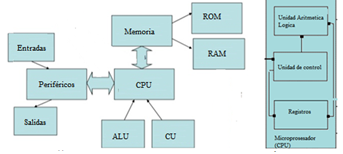
\includegraphics[scale=0.75]{introduccion/imagenes/microcontrolador}
	\textbf{\caption{\small{Diagramas de un microcontrolador (lado izquierdo) y microprocesador (lado derecho)  \cite{veintinueve}.}}}
	\label{Seccion1.5.5:Figura1.12}
\end{figure} 

La idea de utilizar microcontroladores es la tener un módulo específico que se concentre en una tarea repetitiva y de alguna manera dividir el trabajo. 

\begin{figure}[h]
	\centering
	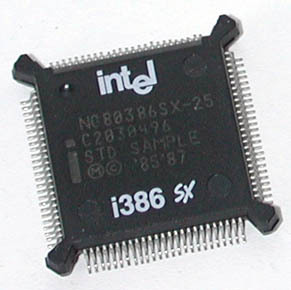
\includegraphics[scale=0.35]{introduccion/imagenes/microprocesador}
	\textbf{\caption{\small{Microprocesador \cite{treinta}.}}}
	\label{Seccion1.5.5:Figura1.13}
\end{figure} 

En la Tabla 1.3 se da la clasificación general de los microcontroladores de acuerdo a sus características principales. \\

	\begin{table}
	\centering
		\begin{tabular}{|p{4cm}|p{7.5cm}|}
			\hline
			Clasificación de los microcontroladores por & Descripción \\
			\hline \hline
			Tamaño de los datos	& 4 bits, 8 bits, 16 bits, 32 bits, 64 bits \\
			\hline
			Arquitectura interna & Von Neumann, Harvard \\
			\hline
			Arquitectura del procesador & CISC (Computador de juego de instrucciones complejo) RISC (Computador de juego de instrucciones reducido) \\		
			\hline
		\end{tabular}
	\textbf{\caption{\small{\textbf{Clasificación de microcontroladores \cite{veintinueve}.}}}}
\end{table}

\textbf{Arquitectura interna de un microcontrolador} \\

Todos los microcontroladores en la actualidad posen dos modelos básicos de arquitectura, denominadas Harvard y Von Neumann, estas arquitecturas tienen diferentes formas de intercambiar los datos \cite{veintinueve}. \\

\begin{itemize}
	\item \textbf{Arquitectura de Von Neumann} \\
	
	Es la arquitectura tradicional de computadoras y microprocesadores, en la cual la CPU está conectada en una memoria única donde se guardan las instrucciones de programas y datos. Los microcontroladores que tienen esta arquitectura internamente soló tienen un bloque de memoria y un bus de datos de 8 bits, los datos se transmiten por este bus llegando a sobrecargarlo ocasionando que la comunicación sea lenta, por otra parte solo permite lectura o escritura de la memoria en cada pulso de reloj. 
	
	\begin{figure}[h]
		\centering
		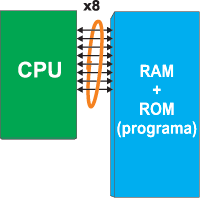
\includegraphics[scale=0.75]{introduccion/imagenes/arquitectura_von}
		\textbf{\caption{\small{Arquitectura Von Neumann \cite{treinta}.}}}
		\label{Seccion1.5.6:Figura1.14}
	\end{figure} 

	\item \textbf{Arquitectura Harvard} \\
	
	Esta arquitectura tiene la CPU conectada a dos memorias (una con las instrucciones y otra con los datos) por medio de dos buses diferentes. Una de las memorias contiene solamente las instrucciones del programa (memoria del programa) y el otro solo almacena los datos (memoria de datos). Ambos buses son totalmente independientes y pueden ser independientes y distintos anchos \cite{treintayuno}. \\
	
	\begin{figure}[h]
		\centering
		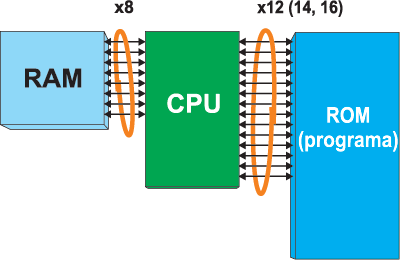
\includegraphics[scale=0.75]{introduccion/imagenes/arquitectura_harvard}
		\textbf{\caption{\small{Arquitectura Harvard \cite{treintayuno}.}}}
		\label{Seccion1.5.6:Figura1.15}
	\end{figure} 

Al tener un bus dedicado a los datos y otro a la memoria del programa, permite que la CPU pueda leer y escribir una instrucción en el mismo pulso de reloj. \\

\end{itemize}

\textbf{Juego de instrucciones} \\

Es el nombre colectivo de todas las instrucciones que tiene un microcontrolador, son instrucciones a nivel máquina que indican al microcontrolador las tareas que debe realizar, cada fabricante personaliza el número de instrucciones que maneja su microcontrolador. \\

\begin{figure}[h]
	\centering
	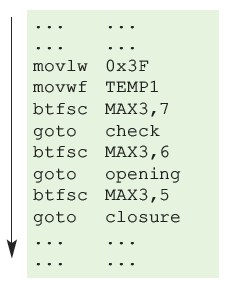
\includegraphics[scale=0.75]{introduccion/imagenes/juego_instrucciones}
	\textbf{\caption{\small{Juego de instrucciones  \cite{treintayuno}.}}}
	\label{Seccion1.5.6:Figura1.16}
\end{figure}

\textbf{Tipos de arquitectura de procesadores} \\

Los microprocesadores basados en una arquitectura CISC disponen de más de 200 instrucciones máquina, siendo estas muy complejas llegando a necesitar más de un ciclo de reloj. La ventaja de tener un juego de instrucciones complejo, es disminuir el tiempo al realizar más de una operación pues éstas en ocasiones se realizan con una sola instrucción. \\

En cuanto a los microprocesadores que utilizan la arquitectura RISC, reconoce y ejecuta pocas instrucciones básicas y realiza operaciones complejas combinando sus instrucciones, cuando se corre una instrucción regularmente solo utiliza un ciclo de reloj, por otra parte, al tener un set de instrucciones más pequeños, ayudan a optimizar los recursos de hardware de un microcontrolador \cite{veintinueve}. 

\subsection{Aplicación Móvil}

Sabemos que la era tecnológica va en aumento y la velocidad con la que evolucionan los dispositivos móviles como lo son: teléfonos celulares, tabletas y Asistentes Personales Digitales (PDA) es cada vez mayor, este impacto tiene su procedencia debido a que la población en su mayoría cuenta con un teléfono celular. \\

El estudio realizado por el Instituto Nacional de Estadística y Geografía (INEGI) en el documento: “ESTADÍSTICAS A PROPÓSITO DEL DÍA MUNDIAL DE INTERNET (17 DE MAYO)”, revela que 77.7 millones de personas usan celular y dos de cada tres usuarios cuentan con un teléfono inteligente (Smartphone), como se muestra en la figura 1.17.

\begin{figure}[h]
	\centering
	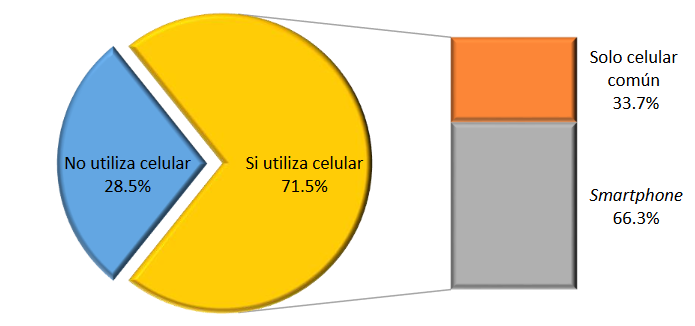
\includegraphics[scale=0.55]{introduccion/imagenes/poblacion}
	\textbf{\caption{\small{Población según condición de uso de celular, por tipo de equipo, 2015($\%$) \cite{treintayuno}.}}}
	\label{Seccion1.5.7:Figura1.17}
\end{figure}

Una aplicación móvil, es un diseño, desarrollo e implementación de un servicio que está pensado para resolver alguna problemática, dicha aplicación se ejecuta en la red y proporciona un valor añadido al cliente. En este escenario el servicio móvil necesita de dos partes: un proveedor de servicios y el usuario del servicio \cite{treintaydos}. \\

Existen dos tipos de aplicaciones móviles: \\
 \begin{itemize}
 	\item \textbf{Aplicaciones móviles web} \\
 	
 	Una aplicación web para móviles, es una aplicación web con formato para teléfonos inteligentes y tabletas, y se accede a través del navegador web del dispositivo móvil. \\
 	
 	\item \textbf{Aplicaciones móviles nativas} \\
 	
 	Una aplicación móvil nativa está construida específicamente para un dispositivo en particular y su sistema operativo. A diferencia de una aplicación web que se accede a través de Internet, una aplicación nativa se descarga desde una tienda virtual y se instala en el dispositivo. \\
 	
 	El desarrollo nativo es el desarrollo de aplicaciones que utilizan las especificaciones de los proveedores del sistema operativo (Google para Android y Apple para IOS) esto implica ajustarse a los lenguajes, frameworks e IDE’s del fabricante o proveedor \cite{treintaytres}.
 	
 \end{itemize}

	   \section{Justificación}


    \chapter{Análisis} 


	   \section{Subtema 1}


	   \section{Métricas y estimación del personal, tiempo y esfuerzo para el desarrollo del prototipo}

Un factor importante de cualquier procedimiento de la ingeniería es la medición. Se pueden usar medidas para comprender mejor los atributos de los modelos que se crean y para valorar la calidad de los productos o sistemas sometidos a ingeniería. Medir es el método a través del cual se determinan números o símbolos a los atributos de las entidades en el mundo real de manera que se les define de acuerdo con reglas claramente determinadas […]. Métrica es una medida cuantitativa del grado en el que un sistema, componente o proceso posee un atributo determinado. \\

Aunque las métricas de producto para el software de computadora son imperfectas, pueden proporcionar una forma sistemática de valorar la calidad con base en un conjunto de reglas claramente definidas. \\

Para el desarrollo del proyecto se ocupará la métrica basada en funciones, la cual se basa en la métrica de punto de función (PF), de modo que puede usarse de manera efectiva como medio para medir la funcionalidad que entra a un sistema. Al usar datos históricos, la métrica PF puede entonces usarse para:

\begin{itemize}
	\item Estimar el costo o esfuerzo requerido para diseñar, codificar y probar el software
	\item Predecir el número de errores que se encontraran durante las pruebas
	\item Prever el número de componentes y/o de líneas fuente proyectadas en el sistema implementado
\end{itemize}

Los puntos de función se derivan usando una relación empírica basada en medidas contables (directas) del dominio de información del software y en valoraciones cualitativas de la complejidad del software. \\

Para calcular los Puntos de Función (PF), se usa la siguiente relación:

\begin{equation}
  PF = conteo \quad total \quad \times \quad[0\ldotp65 + 0\ldotp01 \times \sum(F_i)]
\end{equation}

Donde $conteo\quad total$ es la suma de todas las entradas $PF$ obtenidas de la Tabla 2.1, los $F_i (i=1 \quad al \quad 14)$ son Factores de Ajuste de Valor $(FAV)$ con base en respuestas a las siguientes preguntas: \\

Cada una de estas preguntas se responde usando una escala que varía de 0 (no importante o aplicable) a 5 (absolutamente esencial) \cite{cuarentaydos}.

\begin{table}
	\centering
	\begin{tabular}{|p{1cm}|p{10cm}|p{1cm}|}
		\hline
		1. & ¿El sistema requiere de respaldo y recuperación confiables? & 5\\
		\hline 
		2.	& ¿Se requieren comunicaciones de datos especializadas para transferir información hacia o desde la aplicación? & 5 \\
		\hline
		3. & ¿Existen funciones de procesamiento distribuidas? & 0 \\
		\hline
		4. & ¿El desempeño es crucial? & 5 \\		
		\hline
		5. & ¿El sistema correrá en un entorno operativo existente y enormemente utilizado? & 5 \\
		\hline
		6. & ¿El sistema requiere entrada de datos en línea? & 4 \\
		\hline
		7. & ¿La entrada de datos en línea requiere que la transacción de entrada se construya sobre múltiples pantallas u operaciones? & 5 \\
		\hline
		8. & ¿Los ALI (archivo configuración sistema) se actualizan en línea? & 3 \\
		\hline
		9. & ¿Las entradas, salidas, archivos o consultas son complejos? & 5 \\
		\hline
		10. & ¿El procesamiento interno es complejo? & 5 \\
		\hline
		11. & ¿El código se diseña para ser reutilizable? & 5 \\
		\hline
		12. & ¿La conversión y la instalación se incluyen en el diseño? & 4 \\
		\hline
		13. & ¿El sistema se diseña para instalaciones múltiples en diferentes organizaciones? & 5 \\
		\hline
		14. & ¿La aplicación se diseña para facilitar el cambio y su uso por parte del usuario? & 5 \\
		\hline
		\multicolumn{2}{|l}{Cuenta total $(\sum f_i)$} & 61 \\
		\cline{1-3}
	\end{tabular}
	\textbf{\caption{\small{\textbf{Factores de ajuste de valor \cite{cuarentaydos}.}}}}
\end{table}


Calculo de puntos de función \\

\begin{table}[htb]
	\centering
	\begin{tabular}{|p{3cm}|p{1.2cm}|p{1.2cm}|p{1.4cm}|p{1.4cm}|p{1.2cm}|p{1.2cm}|}
		\hline
		Valor de dominio de información & \multicolumn{6}{c|}{Factor ponderado} \\
		\cline{2-7} 
		& Conteo & Simple & Promedio & Complejo & Factor tomado & Subtotal \\
		\hline \hline
		Entradas de usuario & 5	x & 3 & 4 & 6 & 6 & 30 \\ \cline{2-7}
		\hline 
		Salidas de usuario & 4 x & 4 & 5 & 7 & 7 & 28 \\ \cline{2-7}
		\hline 
		Peticiones de usuario & 2 x & 3 & 4 & 6 & 3 & 6 \\ \cline{2-7}
		\hline 
		Archivos & 1 x & 7 & 10 & 15 & 7 & 7 \\ \cline{2-7}
		\hline 
		Interfaces externas & 2	x & 5 & 7 & 10 & 10 & 20 \\ \cline{2-7}
		\hline 
		\multicolumn{6}{|l}{Conteo total} & 91 \\
		\cline{1-7}
	\end{tabular}
	\textbf{\caption{\small{\textbf{Cálculo de puntos de función \cite{cuarentaydos}.}}}}
	\label{Justificacion:Tabla1.1}
\end{table}

\textbf{Entradas de usuario:} \\

\begin{enumerate}
	\item Lectura temperatura
	\item Lectura frecuencia cardíaca
	\item Lectura acelerómetro
	\item Configuración de frecuencia de lecturas
	\item Configuración de cada sensor
\end{enumerate}

\textbf{Salidas de usuario:} \\

\begin{enumerate}
	\item Señales de las variables a medir
	\item Interpretación de las señales
	\item Identificación de las señales que sobrepasan los límites estimados
	\item Envío de alertas al dispositivo móvil del usuario indirecto
\end{enumerate}

\textbf{Peticiones de usuario:} \\

\begin{enumerate}
	\item Llamar a un centro de salud
	\item Observar las variables en tiempo real
\end{enumerate}

\textbf{Archivos:} \\

\begin{enumerate}
	\item Información de las variables medidas
\end{enumerate}

\textbf{Interfaces externas:} \\

\begin{enumerate}
	\item Aplicación móvil
	\item Brazalete
\end{enumerate}

Una vez que se obtuvieron todos los datos, se sustituye en la formula siguiente: \\

\begin{equation}
PF = conteo \quad total \quad \times \quad[0\ldotp65 + 0\ldotp01 \times \sum(F_i)]
\end{equation}

\begin{equation}
PF = 91 \quad \times \quad[0\ldotp65 + 0\ldotp01 \times (61)] = 114\ldotp66
\end{equation}

Se puede notar que la cantidad de funciones necesarias son 114.66. \\

Tomando en cuenta que un estándar de líneas de código por función en un sistema embebido es de 70 LDC por función, recordando que anteriormente obtuvimos 108.36 funciones, entonces la cantidad de miles de líneas por código (KLDC) está dado por: \\


	   \section{Análisis de requerimientos}

Los requerimientos funcionales son las soluciones que debe cumplir el prototipo para cubrir los objetivos generales. \\

El origen de los requerimientos del prototipo, derivan por una parte del aumento de la población de adultos mayores, las vulnerabilidades que presentan, brindando herramientas que faciliten su cuidado y atención, sin descuidar las actividades que el jefe del hogar debe realizar para solventar los gastos, está a su vez debe tener un precio accesible. \\

La problemática se identificó de informes nacionales e internacionales dedicados al estudio del núcleo familiar, aumento de la población, el riesgo y capacidades diferentes que presentan las personas de la tercera edad y el uso del tiempo de hombres y mujeres de edad avanzada. Los informes fueron obtenidos de organizaciones como OMS, INEGI y Banco Mundial. \\

\begin{itemize}
	\item \textbf{Requerimientos funcionales:}
\end{itemize}

A continuación, se muestran los requerimientos funcionales: \\

\begin{table}
	\centering
	\begin{tabular}{|p{2cm}|p{3cm}|p{6cm}|}
		\hline
		Identificador & Nombre & Descripción \\
		\hline \hline
		RF1 & Alimentar el prototipo & Alimentar el prototipo con 3v o 5v \\
		\hline
		RF2 & Configuración del prototipo & Configurar las características del usuario directo en el microcontrolador así como la frecuencia de lecturas que se realizaran al usuario directo \\
		\hline
		RF3 & Lectura de datos & Obtener las magnitudes medidas por el sensor de temperatura, ritmo cardíaco y acelerómetro \\		
		\hline
		RF4 & Evaluación de la temperatura & Verificar si la temperatura del usuario directo se encuentra entre $(36\ldotp5^{\circ}C)$ y $(37\ldotp2^{\circ}C)$ (de acuerdo a la OMS) \\
		\hline
		RF5 & Evaluación de ritmo cardíaco & Verificar el ritmo cardíaco del usuario directo se encuentra en un rango aceptable de acuerdo a su edad (basadas en mediciones de instituciones médicas) \\
		\hline
		RF6 & Evaluación de la aceleración & Verificar si la magnitud arrojada por el acelerómetro es normal en una persona de la tercera edad \\
		\hline
		RF7 & Emisión de alertas & Informar al usuario indirecto si los parámetros obtenidos han sobrepasado los rangos aceptables \\
		\hline
		RF8 & Prueba de comunicación & Comprobar la comunicación entre los sensores y el microcontrolador, el dispositivo y la aplicación \\
		\hline
		RF9 & Estado del usuario directo & Muestra la aplicación los últimos valores obtenidos por los sensores \\
		\hline
		RF10 & Historial de variables & Almacenar las lecturas obtenidas por los sensores \\
		\hline
	\end{tabular}
	\textbf{\caption{\small{\textbf{Requerimientos funcionales.}}}}
\end{table}

\newpage

\begin{itemize}
	\item \textbf{Requerimientos no funcionales:}
\end{itemize}

Los requerimientos no funcionales no tienen que ver con los objetivos generales de manera directa, pero no se involucran con las funciones primordiales del prototipo, y se identificaron los siguientes: \\

\begin{table}
	\centering
	\begin{tabular}{|p{2cm}|p{3cm}|p{6cm}|}
		\hline
		Identificador & Nombre & Descripción\\
		\hline \hline
		RF1 & Costo & El costo debe ser accesible para el usuario final \\
		\hline
		RF2 & Interfaz & La interfaz debe ser amigable para el usuario \\
		\hline
		RF3 & Alimentación del prototipo & El prototipo debe tener un consumo mínimo de energía \\		
		\hline
		RF4 & Confort del prototipo	& El dispositivo no debe ser incómodo para el usuario directo \\
		\hline
		RF5 & Estabilidad & El prototipo debe ser constante al tiempo que debe emitir las mediciones, conforme se haya configurado la frecuencia de estás \\
		\hline
	\end{tabular}
	\textbf{\caption{\small{\textbf{Requerimientos no funcionales.}}}}
\end{table}

\begin{itemize}
	\item \textbf{Actores del sistema:} 
\end{itemize}

\begin{enumerate}
	\item \textbf{Usuario Directo:} Es la persona portadora del dispositivo, a la cual se estará monitoreando y de quien se obtendrán las lecturas de: temperatura, ritmo cardíaco y caídas.
	\item \textbf{Usuario Indirecto:} Es la persona que tendrá acceso a la aplicación móvil y a quien se le harán las notificaciones en caso de que el usuario directo necesite algún tipo de ayuda
\end{enumerate}

	   \section{Reglas de negocio}

Al identificar las reglas de negocio que el proyecto pretende cumplir, entendiéndolas y poniéndolas en marcha se irán cubriendo los aspectos principales de dicho proyecto y de esta manera se logrará el objetivo principal. \\ 

\begin{itemize}
	\item Informar cuando la magnitud de temperatura del usuario directo salga del rango comprendido entre $(36\ldotp5^{\circ}C)$ y $(37\ldotp2^{\circ}C)$.
	\item Notificar cuando el usuario presente una caída.
	\item Comunicar si el usuario directo presenta una frecuencia cardíaca que ponga en riesgo su salud.
	\item El prototipo debe Identificar cuando las variables medidas salgan del rango estimado.
	\item El prototipo no debe ser invasivo para el usuario directo.
	\item La respuesta del prototipo hacia el usuario indirecto debe ser en tiempo real.
	\item La comunicación debe ser inalámbrica entre el dispositivo y la aplicación.
	\item El dispositivo a utilizar por el usuario directo debe ser lo más pequeño posible.
	\item La aplicación móvil deberá estar disponible para cualquier sistema operativo móvil.
	\item El costo del prototipo debe ser accesible para el usuario.
	\item Los sensores utilizados en el dispositivo deben tener una resolución aceptable.
\end{itemize}
	   \section{An{á}lisis de factibilidad}

A continuación, se describen los estudios de factibilidad: técnica, operacional y económica, para contemplar los recursos humanos y materiales necesarios para que dicho proyecto pueda desarrollarse e implantarse de igual manera se obtendrá una estimación del costo real del proyecto para que pueda realizarse durante un periodo de 10 meses. \\

\subsection{Análisis de factibilidad técnica}

En este apartado abordaremos los recursos de hardware y software necesarios para que el proyecto pueda desarrollarse e implantarse, tomando en cuenta que dichos recursos son necesarios para que el proyecto pueda funcionar de manera correcta. \\

\begin{table}
	\centering
	\begin{tabular}{|p{5cm}|p{1.5cm}|p{6cm}|}
		\hline
		\centering Recurso & \centering Cantidad & \centering Especificaciones\\
		\tabularnewline
		\hline 
		Dispositivo móvil, preferentemente Smartphone, con acceso a internet y con sistema operativo Android & \centering 1 & Este dispositivo se utilizará para recibir las alarmas o alertas en caso de que haya algún problema con el usuario directo \\
		\hline
		Dispositivo Programador NOMADA & \centering 1 & Este programador se utilizará para programar el microcontrolador \\
		\hline
		Computadora portátil con procesador Intel Core i5, 8GB de Memoria RAM, disco duro de 1TB y pantalla LED de 14.0" & \centering 3 & Las computadoras serán utilizadas por los desarrolladores para crear y programar las aplicaciones necesarias para el proyecto \\		
		\hline
		Sensor de temperatura MLX9061 & \centering 1 & Este sensor se utilizará, para medir la temperatura del usuario \\
		\hline
		Sensor acelerómetro MPU-6050 & \centering 1 & Este sensor se utilizará, para medir las caídas que pueda sufrir del usuario \\
		\hline
		Sensor de frecuencia cardíaca MAX30100 & \centering 1 & Este sensor se utilizará, para medir la frecuencia cardíaca del usuario \\
		\hline
		Microcontrolador ATMega 328-PB & \centering 1 & Este dispositivo se utilizará, para recibir las señales de los sensores y enviar la información a la aplicación móvil \\
		\hline
		Módulo Wifi ESP8266 & \centering 1 & Este dispositivo se utilizará, para la comunicación entre el microcontrolador y la aplicación móvil \\
		\hline
	\end{tabular}
	\textbf{\caption{\small{\textbf{Recursos de hardware.}}}}
\end{table}

\begin{table}
	\centering
	\begin{tabular}{|p{4cm}|p{1.5cm}|p{7cm}|}
		\hline
		\centering Recurso & \centering Cantidad & \centering Especificación\\
		\tabularnewline
		\hline 
		JAVA 8.0 o posterior & \centering 1 & Lenguaje de programación para el desarrollo de la aplicación móvil \\
		\hline
		AVR Studio 7 & \centering 3 & Herramienta de desarrollo para programar el microcontrolador AVR \\
		\hline
		ANDROID STUDIO 2.3 & \centering 3 & Herramienta de desarrollo para programar aplicaciones móviles \\		
		\hline
		START UML & \centering 3 & Herramienta de modelado de diagramas UML, para desarrollo del reporte técnico \\
		\hline
		Microsoft Office & \centering 3 & Herramienta para el desarrollo del reporte técnico \\
		\hline
		Sistema Operativo Linux Fedora 24 Server & \centering 1 & Sistema operativo en el cual se recomienda este alojada la aplicación móvil para su correcto funcionamiento \\
		\hline
		Eagle & \centering 1 & Herramienta para el diseño de la placa donde se montaran los sensores \\
		\hline
		Sistema Operativo Windows 10 & \centering 3 & Sistema operativo con los que deberán contar las computadoras para desarrollo \\
		\hline
	\end{tabular}
	\textbf{\caption{\small{\textbf{Recursos de software.}}}}
\end{table}

\subsection{Análisis de factibilidad operativa}

A continuación mencionaremos los requisitos y habilidades con los que debe contar el personal, quienes desarrollarán el proyecto. 

\begin{table}
%	\centering
	\begin{tabular}{|p{2cm}|p{1.5cm}|p{8cm}|}
		\hline
		\centering Recurso & \centering Cantidad & \centering Habilidades y características\\
		\tabularnewline
		\hline 
		Ingenieros en Sistemas & \centering 3 & Persona que cuente con habilidades de programación en aplicaciones móviles, construcción de circuitos, desarrollo de aplicaciones en c/c++, modelado y creación de reportes técnicos, trabajo en equipo y alta disponibilidad \\
		\hline
	\end{tabular}
	\textbf{\caption{\small{\textbf{Recursos humanos.}}}}
\end{table}

\newpage\subsection{Análisis de factibilidad económica}

En este apartado se calcula el costo estimado de desarrollo del proyecto que será elaborado en un periodo de 10 meses y se hará un presupuesto de costos y gastos del proyecto detallado en las siguientes tablas. \\

\begin{table}[htb]
	\centering
	\begin{tabular}{|p{1cm}|p{2cm}|p{1.5cm}|p{1.8cm}|p{1.8cm}|p{1.8cm}|}
		\hline
	    \multicolumn{6}{|c|}{Costos y gastos de recursos humanos del proyecto} \\
		\cline{1-6} \hline
		\centering N$\circ$ & \centering Puesto & \centering Cantidad & \centering Sueldo mensual & \centering Sueldo para 10 meses & \centering Total \\
		\tabularnewline
		\hline 
		\centering 1.- & Líder de proyecto / programador & \centering 3 & \$15,000.00 & \$150,000.00 & \$450,000.00 \\ \cline{1-6}
		\hline 
	\end{tabular}
	\textbf{\caption{\small{\textbf{Costos y gastos de recursos humanos.}}}}
\end{table}

\begin{table}[htb]
	\centering
	\begin{tabular}{|p{1cm}|p{4cm}|p{1.5cm}|p{2cm}|p{2cm}|}
		\hline
		\multicolumn{5}{|c|}{Costos y gastos de recursos materiales de hardware} \\
		\cline{1-5} \hline
		\centering N$\circ$ & \centering Concepto & \centering Cantidad &\centering Costo unitario & \centering Costo total \\
		\tabularnewline
		\hline 
		\centering 1.- & Dispositivo móvil & \centering 1 & \$7,999.00 & \$7,999.00 \\ \cline{1-5}
		\hline 
		\centering 2.- & Dispositivo programador para microcontrolador & \centering 1 & \$420.00 & \$420.00 \\ \cline{1-5}
		\hline 
		\centering 3.- & Computadora portátil & \centering 3 & \$13,146.00 & \$39,438.00 \\ \cline{1-5}
		\hline 
		\centering 4.- & Sensor de temperatura MLX9061 & \centering 1 & \$280.00 & \$280.00 \\ \cline{1-5}
		\hline
		\centering 5.- & Sensor acelerómetro MPU-6050 & \centering 1 & \$90.00 & \$90.00 \\ \cline{1-5}
		\hline 
		\centering 6.- & Sensor frecuencia cardiaca MAX30100 & \centering 1 & \$460.00 & \$460.00 \\ \cline{1-5}
		\hline
		\centering 7.- & Microcontrolador ATMega 328-PB & \centering 1 & \$400.00 & \$400.00 \\ \cline{1-5}
		\hline
		\centering 8.- & Módulo Wifi ESP8266B & \centering 1 & \$120.00 & \$120.00 \\ \cline{1-5}
		\hline
	\end{tabular}
	\textbf{\caption{\small{\textbf{Costos y gastos de recursos materiales de hardware.}}}}
\end{table}

\begin{table}[htb]
	\centering
	\begin{tabular}{|p{1cm}|p{3cm}|p{1.5cm}|p{2cm}|}
		\hline
		\multicolumn{4}{|c|}{Costos y gastos de recursos materiales de software} \\
		\cline{1-4} \hline
		\centering N$\circ$ & \centering Concepto & \centering Cantidad & \centering Costo total \\
		\tabularnewline
		\hline 
		\centering 1.- & Microsoft Office & \centering 3 & \$1,099.00 \\ \cline{1-4}
		\hline 
		\multicolumn{3}{|c|}{Totales} & \$1,099.00 \\ \cline{1-3} 
		\hline
	\end{tabular}
	\textbf{\caption{\small{\textbf{Costos y gastos de recursos materiales de software.}}}}
\end{table}

\begin{table}[htb]
	\centering
	\begin{tabular}{|p{1cm}|p{2cm}|p{4cm}|p{4cm}|}
		\hline
		\multicolumn{4}{|c|}{Costos y gastos de recursos materiales del proyecto} \\
		\cline{1-4} \hline
		\centering N$\circ$ & \centering Concepto & \centering Valor mes & \centering Valor por 10 meses \\
		\tabularnewline
		\hline 
		\centering 1.- & Papelería & \$1,000.00 & \$10,000.00 \\ \cline{1-4}
		\hline 
		\centering 2.- & Otros & \$1,000.00 & \$10,000.00 \\ \cline{1-4}
		\hline
		\multicolumn{2}{|c|}{Totales} & \$2,000.00 & \$20,099.00 \\ \cline{1-2} 
		\hline
	\end{tabular}
	\textbf{\caption{\small{\textbf{Resumen de recursos materiales de proyecto.}}}}
\end{table}

\begin{table}[htb]
		\centering
	\begin{tabular}{|p{1cm}|p{5cm}|p{2.5cm}|p{2.5cm}|}
		\hline
		\multicolumn{4}{|c|}{Gastos generales del proyecto} \\
		\cline{1-4} \hline
		\centering N$\circ$ & \centering Concepto & \centering Valor mes & \centering Valor por 10 meses \\
		\tabularnewline
		\hline 
		\centering 1.- & Electricidad áreas comunes & \$500.00 & \$5,000.00 \\ \cline{1-4}
		\hline 
		\centering 2.- & Agua áreas comunes y oficinas & \$130.00 & \$1,300.00 \\ \cline{1-4}
		\hline
		\centering 3.- & Servicio teléfono oficinas & \$200.00 & \$2,000.00 \\ \cline{1-4}
		\hline
		\centering 4.- & Servicio internet oficinas & \$700.00 & \$7,000.00 \\ \cline{1-4}
		\hline
		\centering 5.- & Servicio de hosting y dominio & \$146.99 & \$1,499.90 \\ \cline{1-4}
		\hline
		\centering 6.- & Renta del lugar de trabajo oficinal & \$5,000.00 & \$50,000.00 \\ \cline{1-4}
		\hline
		\centering 7.- & Servicio de limpieza & \$2,500.00 & \$25,000.00 \\ \cline{1-4}
		\hline
		\multicolumn{2}{|c|}{Totales} & \$9,176.99 & \$91,769.90 \\ \cline{1-2} 
		\hline
	\end{tabular}
	\textbf{\caption{\small{\textbf{Resumen de recursos materiales de proyecto.}}}}
\end{table}

\begin{table}[htb]
		\centering
	\begin{tabular}{|p{5cm}|p{3cm}|p{3cm}|}
		\hline
		\centering Concepto & \centering Mensual & \centering En 10 meses \\
		\tabularnewline
		\hline
		Nómina mensual & \$45,000.00 & \$450,000.00 \\
		\hline 
		Recursos materiales de hardware & \$49,207.00 & 49,207.00 \\
		\hline 
		Recursos materiales de software & \$1,099.00 & \$1,099.00 \\
		\hline
		Recursos materiales & \$2,000.00 & \$20,000.00 \\
		\hline
		Gastos generales del proyecto & \$9,176.99 & \$91,769.90 \\
		\hline
		Totales & \$56,176.99 & \$612,075.90 \\ 
		\hline
	\end{tabular}
	\textbf{\caption{\small{\textbf{Resumen de recursos materiales de proyecto.}}}}
\end{table}

\newpage
	   \newpage\section{An{á}lisis de Riesgos}

En esta sección hablaremos de los riesgos que pueden afectar el desarrollo del prototipo, la probabilidad que de estos ocurran, y el impacto que tienen en el prototipo. El análisis y la gestión de riesgos son una serie de pasos que nos permiten comprender y gestionar la incertidumbre que se tiene en el prototipo \cite{cuarentaycuatro}. \\

Comenzaremos definiendo lo que es un riesgo para poder identificarlos, un riesgo es un problema potencial que afecta al desarrollo del proyecto, este puede pasar o no. \\

Los pasos que realizaremos para analizar y gestionar los riesgos son los siguientes: \\

\begin{itemize}
	\item Identificarlos.
	\item Evaluar la probabilidad de ocurrencia.
	\item Estimar el impacto que tendrían.
	\item Establecer un plan de contingencia para los riesgos de alto impacto.	
\end{itemize}

Los riesgos que se identificaron son los siguientes: \\

\begin{itemize}
	\item R1: Mala organización con los integrantes del equipo.
	\item R2: El usuario no está capacitado para utilizar el producto.
	\item R3: Un integrante del equipo sufra alguna enfermedad grave.
	\item R4: Los sensores no se encuentren en óptimas condiciones a la hora de las pruebas.
	\item R5: La comunicación entre los sensores y el microcontrolador no sea correcta.
	\item R6: El módulo de Wifi no transmita bien los datos.
	\item R7: La comunicación entre la aplicación y hardware no son correctos.
	\item R8: El prototipo no se termine en el tiempo estimado.
	\item R9: El dispositivo móvil no cuenta con las características especificadas para el proyecto.
	\item R10: El usuario directo arruine la pulsera de sensores.
	\item R11: Se presente un inconveniente en el desarrollo por falta de conocimiento.
	\item R12: La alimentación suministrada por las pilas hacia los sensores no sea suficiente para realizar las pruebas mínimas.
	\item R13: El microcontrolador se arruine.
	\item R14: El prototipo no cumpla las expectativas del cliente.
	\item R15: Los sensores no se encuentre calibrados.
\end{itemize}

Una vez que se identificaron los riesgos entre el equipo de trabajo, lo siguiente es estimar la probabilidad de que ocurran, esta probabilidad se toma de los integrantes del equipo pues cada uno tiene en mente las actividades que se deben desarrollar, y los problemas que se pueden presentar. Además, que se identifican los riesgos de acuerdo, al tipo de riesgo y al nivel de impacto que tienen \cite{cuarentaycuatro}. \\

\textbf{Tipo de riesgo} \\

\textbf{Riesgo de rendimiento (Rr):} El grado de incertidumbre con el que el producto encontrará sus requisitos y se adecue para su empleo pretendido. \\

\textbf{Riesgo de coste (Rc):} El grado de incertidumbre que mantendrá el presupuesto del proyecto. \\

\textbf{Riesgo de soporte (Rs):} El grado de incertidumbre de la facilidad del software para corregirse, adaptarse y ser mejorado. \\

\textbf{Riesgo de la planificación temporal (Rpt):} El grado de incertidumbre con que se podrá mantener la planificación temporal y de que el producto se entregue a tiempo. \\

El impacto se considera de acuerdo a los siguientes valores: \\

\begin{enumerate}
	\item Catastrófico.
	\item Critico.
	\item Marginal.
	\item Despreciable.
\end{enumerate}

\begin{longtable}{|p{1cm}|p{1.5cm}|p{2cm}|p{1.2cm}|p{5.5cm}|}
%	\centering
		\hline
		Riesgo & Categoría & Probabilidad & Impacto	& Plan de contingencia \\
		\hline \hline
		R1 & Rpt & 20\%	& 2	& Evaluar las actividades en equipo y asignar actividades faltantes, de acuerdo al cronograma \\
		\hline 
		R2 & Rr & 30\% & 3 & Se realizarán manuales o guías que expliquen el funcionamiento y uso del prototipo \\
		\hline 
		R3 & Rpt & 10\% & 2 & Se dividirá las actividades faltantes con los únicos integrantes del equipo \\
		\hline
		R4 & Rs & 50\% & 3 & Se realizarán pruebas mínimas antes de realizar las pruebas finales, se tendrán repuesto en el caso de que sea necesario cambiarlos \\
		\hline
		R5 & Rs & 30\% & 1 & Se realizarán pruebas entre cada sensor y el microcontrolador, para determinar la posible falla \\
		\hline
		R6 & Rs & 40\% & 2 & Se realizarán pruebas con el módulo de manera individual, y se observarán las posibles fallas que este pueda presentar, para realizar buenas prácticas \\ 
		\hline
		R7 & Rs & 40\% & 1 & Se analizará el hardware de manera individual, una vez que se determine si los resultados son los esperados, evaluaremos la aplicación de acuerdo módulos por los que pasan los datos \\ 
		\hline
		R8 & Rpt & 40\% & 1 & Se organizarán juntas, en las que se evaluara el avance del prototipo y las actividades faltantes, para determinar un plan de acción, para regularizar los tiempos con el cronograma \\ 
		\hline
		R9 & Rs & 20\% & 2 & Se indicará las tecnologías requeridas para el funcionamiento del prototipo \\ 
		\hline
		R10 & Rr & 10\% & 2 & Se pondrán en el manual de usuario, acciones que pongan en riesgo el funcionamiento del prototipo, con el fin de que se tomen en cuenta \\ 
		\hline
		R11 & Rpt & 30\% & 1 & Se realizarán investigaciones previas para dominar el tema.
		Se realizarán juntas con el fin de discutir los temas desconocidos, para después tomar cursos o talleres que nos permitan cubrir ese conocimiento \\ 
		\hline
		R12 & Rr & 30\% & 4 & Se realizarán pruebas una vez que se tenga implementado todo el prototipo, con el fin de analizar la corriente que esté consume, y determinar el arreglo de pilas que se debe utilizar \\ 
		\hline
		R13 & Rr & 10\% & 2 & Comprar varios repuestos para poder cambiarlos, además de analizar el manual para determinar buenas prácticas \\ 
		\hline
		R14 & Rr & 20\% & 2 & Se pensará en las dificultades del cliente indirecto, con el fin de reducir las molestias que pudiese presentar el prototipo \\ 
		\hline
		R15 & Rr & 10\% & 4 & Se implementará un estudio del usuario final con el fin de estudiar las variables, que pudiese presentar su condición actual, se considerará el factor de emisión su frecuencia cardíaca acorde a su edad \\ 
		\hline	
		\caption{Análisis de riesgos \cite{cuarentaycuatro}.}
\end{longtable}

Una vez que se tienen los riesgos se evalúa el impacto y la probabilidad de cada riesgo, mediante la Tabla 2.XVI \\

\begin{table}[htb]
	\begin{tabular}{|p{2cm}|p{1.5cm}|p{2cm}|p{1.6cm}|p{1.5cm}|p{2.1cm}|}
%		\centering
		\hline
		\cellcolor{blue} & \cellcolor{yellow}Impacto & Despreciable & Marginal & Critico & Catastrófico\\
		\cline{2-6}
		\cellcolor{blue} \multirow{2}{2cm}[5mm ]{Probabilidad} & & 4 & 3 & 2 & 1 \\
		\hline
		\cellcolor{blue} Raro & 1 & \cellcolor{green} R15 & \cellcolor{green} R2,R9,R13, & \cellcolor{yellow} R1, R3, R10, R13,R14, & \cellcolor{red} \\
		\hline
		\cellcolor{blue} Moderado & 2 & \cellcolor{yellow} R12 & \cellcolor{yellow} & \cellcolor{red} & \cellcolor{red} R11, R5 \\
		\hline
		\cellcolor{blue} Muy probable & 3 & \cellcolor{yellow} & \cellcolor{yellow} R4 & \cellcolor{red} R6 & \cellcolor{red} R7,R8, \\
		\hline
		\cellcolor{blue} Seguro & 4 & \cellcolor{yellow} & \cellcolor{yellow} & \cellcolor{red} & \cellcolor{red} \\
		\hline
	\end{tabular}
\textbf{\caption{\small{\textbf{Semáforo de riesgos \cite{cuarentaycuatro}.}}}}
\end{table}




%	   \newpage\section{An{á}lisis sensor de Temperatura}

Este apartado pretende explicar los conceptos básicos empleados para entender las variables a medir, explicar el funcionamiento de los sensores y el motivo por el cual se decidió elegir cada sensor. \\

\subsection{Definiciones de temperatura}

\begin{itemize}
	\item La temperatura es la magnitud física que indica que tan caliente o fría esta una sustancia u objeto con respecto a una escala que se toma como referencia.
	\item A nivel molecular la temperatura se define como la energía promedio que desprenden las moléculas que componen un objeto al estar el movimiento.
\end{itemize}

\subsection{Sensores de temperatura}

Este apartado pretende explicar cuáles son las características importantes para elegir un sensor de temperatura en el ámbito eléctrico, y por otro lado las cualidades de diseño del sensor que son aceptables para el prototipo. \\

Existe una gran diversidad de sensores de temperatura, esta diversidad depende mucho del uso que se le pretenda dar. Los sensores considerados una parte están diseñados para el uso médico, mientras que otros son utilizados en diferentes aplicaciones tanto industriales como agrícolas.

\subsection{Definición de las características eléctricas}

Las características eléctricas tomadas en cuenta en la selección de sensores son las siguientes: \\

\begin{itemize}
	\item Exactitud: Es la diferencia entre la magnitud de salida y la magnitud teórica.
	\item Sensibilidad: Es la variación de magnitudes de salida, producidas por el sensor al percibir una magnitud de entrada. 
	\item Campo de medida: Es el rango de valores de la magnitud, que puede percibir el sensor, el rango se encuentra entre el valor mínimo aceptable y el valor máximo aceptable.
	\item Resolución: Es el valor mínimo entre los valores que puede distinguir el sensor.
	\item Tiempo de respuesta: Es el tiempo que tarda el sensor al emitir la señal de salida, una vez que ha recibido la de entrada.
\end{itemize}

En la Tabla 2.32 se muestran algunos sensores que hay en el mercado, se eligieron de acuerdo al campo de medición, su sensibilidad, tiempo de respuestas, su salida y por último el precio. \\

\begin{table}[htb]
	\begin{tabular}{|p{1.8cm}|p{1.8cm}|p{1.3cm}|p{1.8cm}|p{2.3cm}|p{1.3cm}|}
		\hline 
		\centering Sensor & \centering Tiempo de Respuesta & \centering Salida & \centering Resolución & \centering Campo de medición & \centering Precio \\ 
		\tabularnewline
		\hline 
		Amphenol MA100 & En el aire 15s \par En agua 2.0s & Resistiva & 1$^{\circ}$C & 0$^{\circ}$C a 50$^{\circ}$C  & \$8.00 \\ 
		\hline 
		Amphenol MA200 & En el aire 35s \par En agua 0.6s & Resistiva & 1$^{\circ}$C & 0$^{\circ}$C a 50$^{\circ}$C  & \$8.00 \\ 
		\hline 
		Amphenol MA300 & En el aire 45s \par En agua 2s & Resistiva & 1$^{\circ}$C & 0$^{\circ}$C a 50$^{\circ}$C  & \$8.00 \\  
		\hline 
		LM334 & --- & Corriente & 1.04$^{\circ}$C & 0$^{\circ}$C a 70$^{\circ}$C & \$47.5 \\ 
		\hline 
		LM35 & 1s & Voltaje & 10mv/$^{\circ}$C & -55$^{\circ}$C a 150$^{\circ}$C & \$42.00 \\ 
		\hline 
		MLX90614 & 5ms & Voltaje & 0.2$^{\circ}$C & -70$^{\circ}$C a 380$^{\circ}$C & \$280.00 \\ 
		\hline 
	\end{tabular} 
\textbf{\caption{\small{\textbf{Características de sensores de temperatura.}}}}
\end{table}


Analizando las propiedades eléctricas de los sensores elegimos el sensor MLX90614 por su sensibilidad de 0.2$^{\circ}$C ya que para nuestro proyecto es necesario medir con una sensibilidad menor a 1$^{\circ}$C, debido a que las vulnerabilidades se presentan al tener temperaturas que pasan en $\pm$0.2$^{\circ}$C el rango aceptable (36.5$^{\circ}$C a 37.2$^{\circ}$C), otra característica que nos es importante es el tiempo de respuesta del sensor que es en el orden de los milisegundos, la comunicación es otro aspecto que se consideró, para poder comunicarlo con el microcontrolador, en este caso es $I^2 C$, y por ultimo tenemos un precio aceptable y una alimentación estándar de 3v a 5v.

\subsection{Sensor MLX90614}


En este aparto explicaremos el funcionamiento del sensor de temperatura MLX90614 indicando el funcionamiento interno para medir la temperatura. \\

El sensor de temperatura MLX90614 es un sensor de temperatura infrarrojo, el cual capta la temperatura promedio de un lector infrarrojo que mide la energía desprendida por los objetos. Esté sensor infrarrojo tiene una conexión en serie de dos termopares, una se encuentra dentro soporte del chip conectada con un sensor que mide la temperatura del chip, y la otra está colocada en una membrana delgada que está unida con el lector infrarrojo esté absorbe la radiación de la membrana, ya sea caliente o fría \cite{cuarentaycinco}.

\begin{figure}[h]
	\centering
	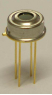
\includegraphics{analisis/imagenes/sensor_temperatura}
	\textbf{\caption{\small{Sensor de temperatura MLX9614 \cite{cuarentaycinco}.}}}
	\label{fig:sensortemperatura}
\end{figure}

A continuación, explicaremos que es un termopar y cómo es que funciona, para poder entender cómo es que funciona en sensor MLX90614.
Un termopar es una unión de dos metales distintos unidos en un extremo, cuando a la unión se le presenta una temperatura distinta a la temperatura de la unión se genera un voltaje muy pequeño (efecto Seebeck) del orden de los milivolts, esté aumenta conforme la temperatura se incrementa (no es lineal), dependiendo del tipo de termopar existe una relación temperatura-voltaje. \\

Son utilizadas como sensores de temperatura, el principal inconveniente es la necesidad de compensar a cero, esto se debe a que, al tomar las lecturas en el otro extremo del termopar, se une con otro metal distinto (creando otro termopar) produciendo otro voltaje, el cual es proporcional a la temperatura del ambiente por lo que es necesario medir la temperatura en la unión donde se realiza la lectura, utilizando un sensor que obtenga la temperatura del ambiente. Las dos temperaturas de suman para crear la compensación y así obtener la temperatura real. \\

En la figura 2.4 se muestra los puntos de intersección entre los metales, los puntos en los que se obtiene diferentes temperaturas, siendo T la temperatura del objeto y Ta la temperatura del ambiente.

\begin{figure}
	\centering
	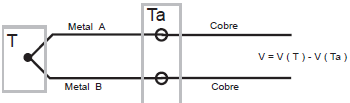
\includegraphics{analisis/imagenes/esquema_termopar}
	\textbf{\caption{\small{Esquema de un termopar (V es el voltaje total obtenido por un volmetro) \cite{cuarentayseis}.}}}
	\label{fig:esquematermopar}
\end{figure}

V(Ta) es el voltaje obtenido por la unión del metal A y el cobre \\

De tal forma que se tienen tres uniones la unión del metal A y metal B, la unión del cobre con el metal B y la unión del metal A con el cobre. Teniendo la siguiente ecuación. \\

\begin{equation}
	V_{Total} \quad = \quad V_{AB(T)} \quad - \quad V_{CuA(Ta) \quad - \quad V_{CuB(Ta)}}
\end{equation}

\begin{equation}
	V_{Total} \quad = \quad V_{AB(T)} \quad - \quad[V_{CuA(Ta) \quad - \quad V_{CuB(Ta)}}]
\end{equation}

\begin{equation}
	V_{Total} \quad = \quad V_{AB(T)} \quad - \quad V_{AB(Ta)}
\end{equation}

\begin{equation}
V_{AB(T)} \quad = \quad V_{Total} \quad - \quad V_{AB(Ta)}
\end{equation}

Posteriormente una vez que se tiene esta ecuación se busca en la tabla del termopar el voltaje $V_{AB(Ta)}$ de acuerdo a la temperatura ambiente, obteniendo el voltaje $V_{AB(T)}$ se puede saber la temperatura de la unión AB, buscando en la tabla del termopar AB, que temperatura corresponde al voltaje $V_{AB(T)}$. \\

Una vez explicado el funcionamiento de un termopar podremos entender ¿Cómo es que mide la temperatura el sensor MLX90614? El sensor MLX90614 tiene internamente dos sensores para medir la temperatura, estos sensores están conectados por medio de un termopar, la primera unión es con el sensor infrarrojo (la membrana) y la segunda con un sensor que mide la temperatura del ambiente, para posteriormente calcular la compensación del termopar y calcular la temperatura del infrarrojo \cite{cuarentayseis}. \\

La señal emitida por el termopar responde a la siguiente ecuación:

\begin{equation}
V_{Ir(Ta,To)} \quad = \quad A \quad \ast \quad (To^4 \quad - \quad Ta^4)
\end{equation}

Donde: \\

\begin{itemize}
	\item $V_{Ir(Ta,To)}$ es el voltaje de respuesta del termopar.
	\item $A$ es la sensibilidad total del infrarrojo.
	\item $To$ es la temperatura obtenida por el infrarrojo.
	\item $Ta$ es la temperatura del ambiente.
\end{itemize}

El principio de los sensores infrarrojos es la radiación infrarroja, está es la parte de la luz solar que se descompone al reflejar la luz solar a través de un prisma, la cual pose energía, teniendo relación con el espectro electromagnético. \\

La energía desprendida por la radiación del campo electromagnético se puede medir mediante una relación con las curvas emitidas por un cuerpo oscuro o negro (emisividad), mientras que los objetos con una temperatura por encima del cero absoluto irradian energía \cite{cuarentaysiete}.

\begin{figure}
	\centering
	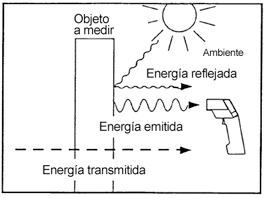
\includegraphics{analisis/imagenes/factor}
	\textbf{\caption{\small{Factor de emisión \cite{cuarentaysiete}.}}}
	\label{fig:factor}
\end{figure}

La cantidad de energía crece de manera proporcional a la cuarta potencia de la temperatura, es por ello que en la ecuación 2.20 las temperaturas $(To^4 \quad - \quad Ta^4)$, en cuanto a A es un factor de emisión que se obtuvo de la relación de las radiaciones que emite un cuerpo gris y un cuerpo negro a igual que la temperatura, estos cuerpos tienen el mismo factor de emisión  en todas las longitudes de onda, por el contrario un cuerpo diferente del gris y el negro cambia su factor de emisión con respecto a la longitud de onda. \\

La temperatura del sensor es necesaria para medir la temperatura del chip, una vez que mide la temperatura del objeto y el ambiente, se calcula la temperatura del chip, los cálculos se realizan por el DPS (Procesador de señal digital) produciendo salidas digitales lineales proporcionales a las temperaturas medidas. \\

Temperatura ambiente \\

El sensor calcula la temperatura mediante termopares y sensores de temperatura internos, todas las condiciones de los sensores y los datos procesados se manejan dentro del chip, mientras que las lecturas de la temperatura del sensor se encuentran en la memoria de acceso aleatorio (RAM) \cite{cuarentaycinco}. \\

La resolución de la temperatura calculada es de 0.02$^{\circ}$C debido a que el convertidor analógico digital (ADC) es de 17 bits, cada bit representa 0.02$^{\circ}$C, el sensor esta calibrado de fábrica con un rango de -40$^{\circ}$C a +125$^{\circ}$C, el valor digital de la temperatura ambiente se encuentra en la RAM en la celda 0x06. \\

Los valores de las temperaturas se encuentran en un formato hexadecimal, la fórmula para obtener la temperatura ambiente en grados $^{\circ}$K es la siguiente:

\begin{equation}
	Ta \quad = \quad {(Valor \quad del \quad registro \quad 0\times06)}_{10} \quad \ast \quad 0\ldotp02
\end{equation}

\begin{itemize}
	\item $Ta$ es el valor de la temperatura ambiente en grados Kelvin.
	\item Es el valor del registro después de convertir de hexadecimal a decimal.
	\item 0.02 es el valor de cada bit.
\end{itemize}

Ejemplos: \\

Tenemos que el valor de la temperatura es 0x2DE4 y se desea saber la temperatura en grados Kelvin como Celsius. \\

\begin{itemize}
	\item El primer pasó el convertir de hexadecimal a decimal el valor del registro.
\end{itemize}

Para convertir de hexadecimal a decimal se utiliza la base 16 y la base 10, multiplicamos cada dígito con el valor de la potencia base dieciséis que le corresponde, siendo el menos significativo el dígito de la derecha. \\

\begin{equation}
Valor \quad digital \quad = \quad 4\ast16^0 \quad + \quad 14\ast16^1 \quad + \quad 13\ast16^2 \quad + \quad 2\ast16^2 
\end{equation}

\begin{equation}
Valor \quad digital \quad = \quad 4 \quad + \quad 224 \quad + \quad 3328 \quad + \quad 8192 
\end{equation}

\begin{equation}
Valor \quad digital \quad = \quad {11748}_{10}  
\end{equation}

El segundo paso es multiplicar la resolución obtenida por el valor digital, obteniendo la temperatura en grados Kelvin, para pasarlos a Celsius se resta 273. \\

\begin{equation}
Ta \quad = \quad 11748 \quad \ast \quad 0\ldotp02
\end{equation}

\begin{equation}
Ta \quad = \quad 234\ldotp96^{\circ}K
\end{equation}

\begin{equation}
Ta \quad = \quad 234\ldotp96 \quad - \quad 273
\end{equation}

\begin{equation}
Ta \quad = \quad - 38\ldotp04^{\circ}C
\end{equation}

El valor mínimo de medición de la temperatura del ambiente es -38.2$^{\circ}$C y el valor máximo medido es 125$^{\circ}$C. \\
 
Temperatura Objeto \\

La temperatura del objeto se encuentra en la celda 0x07, se calcula de la misma manera que la del ambiente, el bit más significativo indica un error, al medir una temperatura que sobre pase los 382.19$^{\circ}$C o en su valor hexadecimal 0x7FFF. \\

Para obtener las mediciones de temperatura, el sensor realiza cálculos, y el resultado lo obtiene lineal, estos pasos se realizan en el núcleo del sensor (en el chip), se ejecuta un programa de la memoria de solo lectura (ROM) antes de encender o de resetear, el chip inicia con los datos de calibración, durante esta fase se selecciona el número de sensor infrarrojo que se utilizará y se decide el rango de temperatura que tendrá en sensor, las rutinas de medición, compensación y la muestra de la  temperatura lineal se corren dentro del término bucle \cite{cuarentaycinco}. \\

El sensor de temperatura utiliza los siguientes filtros para acondicionar las lecturas de temperatura: \\

Filtro Pasa-banda \\

Un filtro pasa-banda permite pasar las frecuencias que están situadas en una determinada banda de frecuencia, es decir entre dos determinadas frecuencias y rechaza las frecuencias fuera de esa banda. \\

Filtros digitales \\

Un filtro digital se puede definir como un proceso computacional o algoritmo mediante el cual una señal digital es transformada en una segunda secuencia de muestras. \\

Respuesta impulsional \\

Es la relación de un filtro a un impulso que se envía a su entrada, la respuesta impulsional caracteriza   a un filtro en el dominio temporal. El funcionamiento de un filtro digital consiste en sumar una señal de entrada a su salida o viceversa. \\

Filtros digital IR y IIR \\

El filtro IR (Respuesta impulsional finita) retarda ligeramente una copia de la señal de entrada (uno o varios periodos) y la suma a la señal de respuesta del filtro \cite{cuarentayocho}. \\ 

\begin{figure}[h]
	\centering
	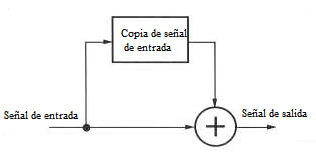
\includegraphics{analisis/imagenes/principio_filtro}
	\textbf{\caption{\small{Principio filtro FIR \cite{cuarentayocho}.}}}
	\label{fig:principiofiltro}
\end{figure}

El filtro digital IIR (Respuesta impulsional infinita) procesa una señal de entrada, la señal obtenida se combina con la de entrada.

\begin{figure}
	\centering
	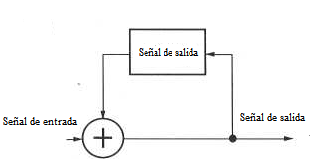
\includegraphics{analisis/imagenes/filtro_iir}
	\textbf{\caption{\small{Principio filtro IIR \cite{cuarentayocho}.}}}
	\label{fig:filtroiir}
\end{figure}

Los filtros se pueden describir mediante ecuaciones que relacionan la señal de entrada con una señal de salida en el domino digital. De manera que la salida del filtro se especifica como un resultado de sumas, restas y multiplicaciones de muestras de entradas actuales y anteriores. \\

Ecuación de los filtros digitales FIR \\

Se puede definir como la combinación lineal de muestras de la entrada presente o pasadas, se expresa de la siguiente forma:

\begin{equation}
	y[n] \quad = \quad a0 \cdot x[n] \quad + \quad a1 \cdot x[n - 1] \quad + \quad a2 \cdot x[n - 2] \quad + \ldots + \quad aN \cdot x[n - N]
\end{equation}

Esta ecuación expresa que la muestra actual de la salida $y[n]$ es igual a la suma de las muestras de la entrada actual $x[n]$ multiplicada por el factor $a0$ y de la muestra anterior $x[n – 1]$ multiplicando por el factor $a1$, y de todas las muestras anteriores hasta el instante $[n - N]$ multiplicado por su correspondiente factor. Donde los factores modifican las características de la señal \cite{cuarentayocho}. \\

Señal digital: \\

\begin{equation}
	x \quad = \quad \{1,0,0,0,0,0,0,\ldots\}
\end{equation}

Señal de salida: \\

\begin{equation}
x \quad = \quad \{a0,a1,a2,a3,\ldots,aN,0,0,0,\ldots\}
\end{equation}

Ecuación de filtro digital IIR \\

Los filtros IIR se distinguen de los filtros FIR por la presencia de una recursividad, la señal de salida del filtro retroalimenta el filtro, esté método permite implementar filtros con respuesta más compleja y con menos datos, al retroalimentar la entrada la respuesta impulsional tiene una duración potencial infinita. \\

\begin{equation*}
	\begin{split}
	y[n] \quad = \quad a0 \cdot x[n] \quad + \quad a1 \cdot x[n - 1] \quad + \quad a2 \cdot x[n - 2] \quad + \ldots + \quad \\ aN \cdot x[n - N] \quad + \quad - \quad b1 \cdot y[n-1] \quad - \quad b2 \cdot y[n-2] \quad - \quad \\ b3 \cdot y[n-3]  \quad \ldots \quad - \quad bM \cdot y[n-M]
	\end{split}		
\end{equation*}

Esta ecuación expresa que la salida es función de N+1 muestras de la entrada (actuales y N anteriores), así como de M muestras anteriores de salida. \\

Diferencia entre los filtros digitales \\

Los filtros FIR ofrecen en general una respuesta de fase más lineal y no entran jamás en oscilación, pero requieren de un gran número de muestras haciéndolos más caros computacionalmente, mientras que los filtros IIR son muy eficaces y pueden proporcionar pendientes de corte muy pronunciadas, pero tienden a entrar en resonancia\cite{cuarentayocho}. \\

Los procesos que se realizan en el sensor se dividen en 3 partes: \\

Desviación del infrarrojo \\

\begin{itemize}
	\item Se mide la desviación con la FIR, fijando la longitud de la respuesta del filtro.
	\item Agrega al filtrado la IIR fijando su longitud, el resultado es almacenado dentro de la RAM en la variable (registro) $IR_{os}$.
	\item Se obtiene otra medida con FIR del filtro, fijando la longitud de la respuesta.
	\item Compensación de la desviación.
	\item Se agrega un proceso adicional programando la longitud IIR, el resultado se almacena dentro de la RAM en $IR_G$.
	\item Se calcula la compensación obtenida, el resultado se almacena dentro de la RAM en $K_G$.
\end{itemize}

Temperatura del Objeto \\

Estos son los procesos que realizan para obtener la temperatura del objeto, el sensor MLX90614 tiene dos sensores infrarrojos internos. \\

\begin{itemize}
	\item Medición del sensor infrarrojo se programa la longitud FIR del filtro.
	\item Compensación de la desviación.
	\item Gana compensación.
	\item Se filtra, programando la longitud IIR del filtro, se almacena el resultado dentro de la RAM en la dirección 0x04 en $IR1_D$.
	\item El cálculo de la temperatura del objeto, se almacena en la dirección 0x07 en $T_{02}$.
	
\end{itemize}

El mismo procedimiento se realiza con el segundo sensor infrarrojo \cite{cuarentaycinco}.


%	   \newpage\section{An{á}lisis sensor Aceler{ó}metro}

En este apartado abordaremos el análisis del sensor acelerómetro que es ampliamente utilizado para detectar cuando una persona sufre una caída; de acuerdo a la investigación se deberán responder las siguientes preguntas: ¿cómo determinamos qué una persona está cayendo?, ¿cuáles son los rangos en los que se establece que una persona sufrió una caída?, ¿cuáles son los motivos por los que se seleccionó el acelerómetro \textbf{MPU-6050}? y por último, ¿cuál es el funcionamiento y las características principales del acelerómetro \textbf{MPU-6050}?. \\

\subsection{Etapas de una caída}

Una caída comprende 4 etapas, en las cuales se observa una aceleración diferente y las etapas críticas tienden a ser los rangos de evaluación para definir si se sufrió o no dicha acción. A continuación, se describen dichas etapas \cite{cuarentaynueve}:

\begin{figure}[h]
	\centering
	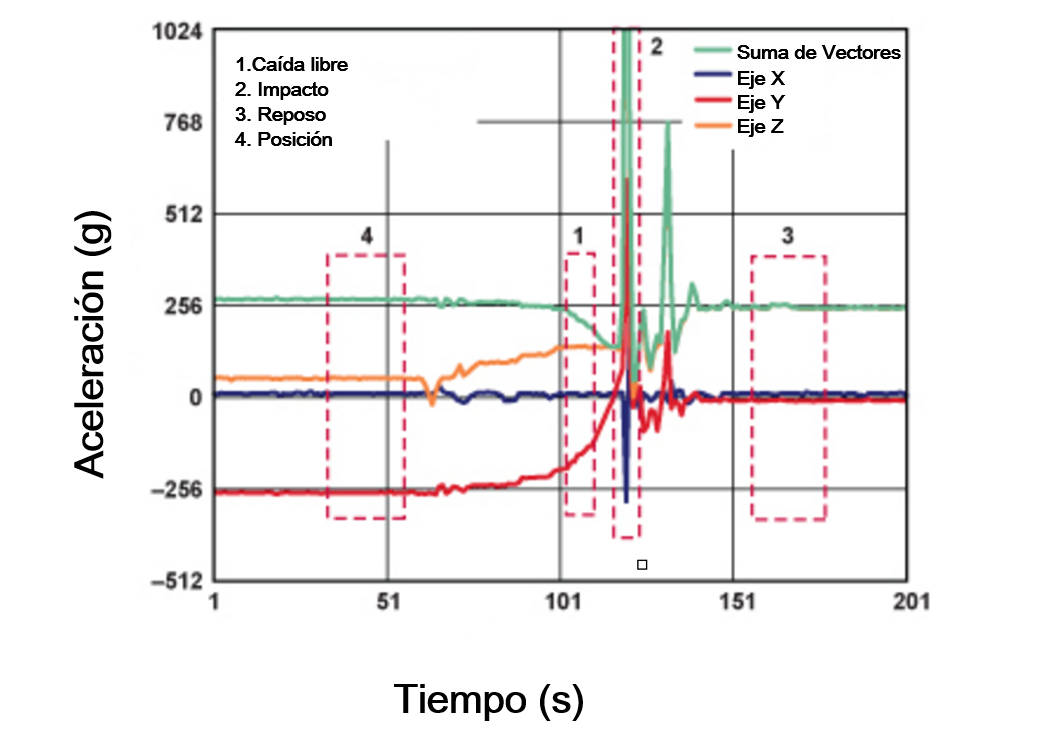
\includegraphics[scale=0.35]{analisis/imagenes/etapas_caida}
	\textbf{\caption{\small{Gráfica 2.1 Puntos de interés en la señal que muestra: (a) posturas al sufrir una caída y (b) actividades cotidianas \cite{cuarentaynueve}.}}}
	\label{fig:sensorcaida}
\end{figure}

\begin{itemize}
	\item \textbf{Caída libre}: Cuando una persona pierde el equilibrio se dirige hacia el suelo con un movimiento de caída libre y es justo donde se da el primer cambio en la señal; en esta etapa se contempla el fenómeno de gravedad y la suma vectorial de la aceleración se reflejará menor que 1g y mayor que $0g (1g > a > g)$. 
	\item \textbf{Impacto}: El cuerpo tendrá un choque con el suelo, pared u objeto, en esta etapa la señal tendrá un cambio significativo teniendo un pico muy elevado con valores en la aceleración de entre $2g y 12g$.
	\item \textbf{Reposo}: El cuerpo humano, después de caer y hacer impacto, no puede levantarse de inmediato; por lo que permanece en una posición inmóvil durante un período de tiempo (este puede ser corto o largo dependiendo de la gravedad de la caída).
	\item \textbf{Posición final}: Después de una caída, el cuerpo de la persona estará en una orientación diferente a la anterior, por lo que la aceleración estática en tres ejes será diferente de la situación inicial antes de la caída. Se hace un muestreo de la aceleración antes (muestreo inicial) y después (muestreo final) de la caída, se comparan los datos de muestreo y se evalúa; si la diferencia entre los datos de muestreo y supera un umbral de $0,7 g$ se declara como caída.
\end{itemize}

\subsection{Algoritmo basado en umbrales y orientación}

Simplemente se basa en detectar las cuatro etapas de las caídas: caída libre, impacto, reposo y posición final.	Se describirá el siguiente algoritmo el cual se abordará en este proyecto para detectar las caídas.

\begin{figure}[h]
	\centering
	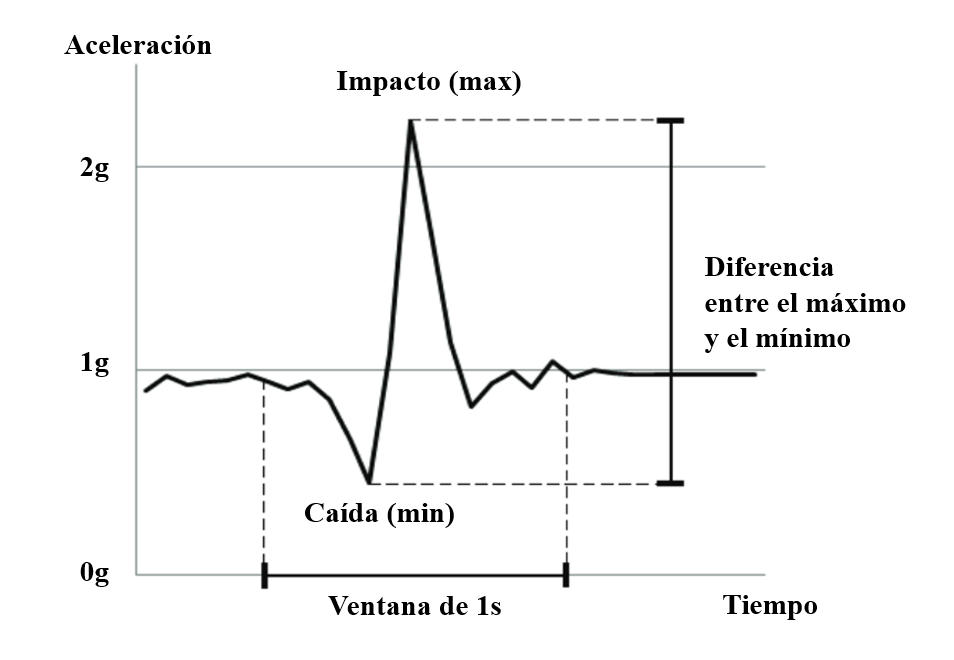
\includegraphics[scale=0.35]{analisis/imagenes/aceleracion}
	\textbf{\caption{\small{Gráfica 2.2 Patrón de la aceleración durante una caída \cite{cincuenta}.}}}
	\label{fig:sensorcaida2}
\end{figure}

\begin{enumerate}
	\item Un acelerómetro registra que una persona en reposo tiene de $1g$ (gravedad de la Tierra) de aceleración y durante la caída libre dicha aceleración tiende a 0 g. Cuando una persona comienza a caer, la aceleración disminuye de $1g \quad a \quad 0.5g$ aproximadamente (nunca se logra caída libre perfecta). 
	\item Tras el impacto con el suelo, se mide un alto y bajo aumento en la aceleración, lo cual nos da un pico muy largo.
	\item En el umbral, se utiliza la longitud del vector de aceleración, ignorando la dirección de la aceleración. En el lapso de un segundo se mide la aceleración máxima y mínima, si la diferencia entre estas aceleraciones: máxima y mínima es mayor de 1g y la máxima se produce después de la mínima, se declara que se ha producido una caída. 
	\item Sea $z$ el eje apuntando hacia abajo cuando la persona está de pie en posición vertical. El ángulo entre el vector de aceleración y el eje $z$, indica la orientación de la persona, y se calcula mediante la siguiente fórmula: 
\end{enumerate}

\begin{equation}
cos\phi \equiv \frac{{\alpha}_{z}}{{\alpha}_{x^2}+{\alpha}_{y^2}+{\alpha}_{z^2}}
\end{equation}

Puesto que cada persona tiene su postura característica y el acelerómetro puede no siempre ser usado exactamente de la misma manera, la orientación promedio de cada persona durante 15 segundos de caminar se mide como ${\phi}_{0}$. Posteriormente, cuando se mide una nueva orientación $\phi$, se normaliza como sigue: ${\phi}_{norm} = \phi – {\phi}_{0}$. Una persona es considerada orientada hacia arriba, si $-30^{\circ} < {\phi}_{norm} < 30^{\circ}$. Por lo cual, si se ha detectado una aceleración que supera el umbral como se ha descrito anteriormente, y la orientación de la persona durante 10 segundos no es en posición vertical, se declara que se ha producido una caída \cite{cincuenta}.

\subsection{Selección y tabla comparativa de acelerómetros}

El acelerómetro seleccionado fue el MPU-6050, de acuerdo a la investigación en la tabla comparativa, esto fue porque incluye un giroscopio, su tipo de interfaz es digital I$^{2}$C, el costo es promedio comparado con los demás, además de tener un diseño para el bajo consumo de energía, de estas características podemos resaltar que es ampliamente usado en: teléfonos inteligentes, tabletas y sensores portátiles. \\

\begin{table}[htb]
	\centering
	\begin{tabular}{|p{1cm}|p{5cm}|p{2.5cm}|p{2.5cm}|p{2.5cm}}
		\hline
		\multicolumn{5}{|c|}{Tabla comparativa de acelerómetros} \\
		\cline{1-5} \hline
		Modelo & MPU-6050 & ADXL345 & MMA8451Q & LIS331HH \\
		\hline 
		Fabricante & Inven Sense & Analog Devices & Freescale & STMicroelectronics \\ \cline{1-5}
		\hline 
		Salida & Digital 8 bits & Digital de 12 bits & Digital 13 bits & Digital 16 bits \\ \cline{1-5}
		\hline
		Interfaz de comunicación & I2C & SPI, I2C & I2C & I2C \\ \cline{1-5}
		\hline
		Rango de medición & ±2g, ±4g, ±8g, ±16g & ±16 & +/- 8g & +/- 24g \\ \cline{1-5}
		\hline
		Dimensión & 4mm x 4mm x 0.9mm & 3mm x 5mm x 1mm & 3mm x 5mm x 1mm & 3mm x 5mm x 1mm \\ \cline{1-5}
		\hline
		Ejes & 3 & 3 & 3 & 3 \\ \cline{1-5}
		\hline
		Precisión & 1mg/LSB & 4 mg/LSB & 0.98 g/LSB & 3 mg/LSB (a +/-12g) \\ \cline{1-5}
		\hline
		Alimentación & 2.375V a 3.46V & 2V a 3.6V & 1.95V a 3.6V & 2.16V a 3.6V \\ \cline{1-5} 
		\hline
		Corriente Máxima & & 40uA & 165uA & 10uA \\ \cline{1-5} 
		\hline
		Características adicionales & Incluye giroscopio & & & \\ \cline{1-5} 
		\hline
		Frecuencia de muestreo & Hasta 400kHz & Hasta 3200 Hz & Hasta 800 Hz & Hasta 1 KHz \\ \cline{1-5} 
		\hline
		Rango de temperatura & -40$^\circ$C a +85$^\circ$C & -40$^\circ$C a +85$^\circ$C & -40$^\circ$C a +85$^\circ$C & -40$^\circ$C a +85$^\circ$C \\ \cline{1-5} 
		\hline
		Calibración & Programable & De Fábrica & De Fábrica & De Fábrica \\ \cline{1-5} 
		\hline
		Montaje superficial & si & si & si & si \\ \cline{1-5} 
		\hline
		Costo & \$3.99 & \$6.93 & \$2.16 & \$5.97 \\ \cline{1-5} 
		\hline
	\end{tabular}
	\textbf{\caption{\small{\textbf{Escenarios y posturas en los que el acelerómetro realizará muestreo.}}}}
\end{table}

\subsection{Características, especificaciones y funcionamiento interno del acelerómetro MPU-6050}

El acelerómetro MPU-6050 cuenta con un acelerómetro y un giroscopio internos, este dispositivo es altamente usado en aplicaciones basadas en video, estabilización de imágenes, seguridad en autenticación, reconocimiento de gestos, control de movimiento, sensores para la salud, sensores para condición física, sensores para deporte y juguetes. En el siguiente apartado se mostrarán las características, diagrama a bloques y la descripción con las que cuenta dicho dispositivo.

\begin{itemize}
	\item \textbf{Características}
\end{itemize}

En la tabla 2.XXXIV se marcarán las características principales para el dispositivo. \\

\begin{table}[htb]
	\begin{tabular}{|p{1.8cm}|p{1.8cm}|p{1.3cm}|p{1.8cm}|p{2.3cm}|p{1.3cm}|}
		\hline 
		Sensor & Tiempo de Respuesta & Salida & Resolución & Campo de medición & Precio \\ 
		\hline 
		Amphenol MA100 & En el aire 15s \par En agua 2.0s & Resistiva & 1$^{\circ}$C & 0$^{\circ}$C a 50$^{\circ}$C  & \$8.00 \\ 
		\hline 
		Amphenol MA200 & En el aire 35s \par En agua 0.6s & Resistiva & 1$^{\circ}$C & 0$^{\circ}$C a 50$^{\circ}$C  & \$8.00 \\ 
		\hline 
		Amphenol MA300 & En el aire 45s \par En agua 2s & Resistiva & 1$^{\circ}$C & 0$^{\circ}$C a 50$^{\circ}$C  & \$8.00 \\  
		\hline 
		LM334 & --- & Corriente & 1.04$^{\circ}$C & 0$^{\circ}$C a 70$^{\circ}$C & \$47.5 \\ 
		\hline 
		LM35 & 1s & Voltaje & 10mv/$^{\circ}$C & -55$^{\circ}$C a 150$^{\circ}$C & \$42.00 \\ 
		\hline 
		MLX90614 & 5ms & Voltaje & 0.2$^{\circ}$C & -70$^{\circ}$C a 380$^{\circ}$C & \$280.00 \\ 
		\hline 
	\end{tabular} 
\textbf{\caption{\small{\textbf{Características de sensores de temperatura.}}}}
\end{table}


Analizando las propiedades eléctricas de los sensores elegimos el sensor MLX90614 por su sensibilidad de 0.2$^{\circ}$C ya que para nuestro proyecto es necesario medir con una sensibilidad menor a 1$^{\circ}$C, debido a que las vulnerabilidades se presentan al tener temperaturas que pasan en $\pm$0.2$^{\circ}$C el rango aceptable (36.5$^{\circ}$C a 37.2$^{\circ}$C), otra característica que nos es importante es el tiempo de respuesta del sensor que es en el orden de los milisegundos, la comunicación es otro aspecto que se consideró, para poder comunicarlo con el microcontrolador, en este caso es $I^2 C$, y por ultimo tenemos un precio aceptable y una alimentación estándar de 3v a 5v.

\subsection{Sensor MLX90614}


En este aparto explicaremos el funcionamiento del sensor de temperatura MLX90614 indicando el funcionamiento interno para medir la temperatura. \\

El sensor de temperatura MLX90614 es un sensor de temperatura infrarrojo, el cual capta la temperatura promedio de un lector infrarrojo que mide la energía desprendida por los objetos. Esté sensor infrarrojo tiene una conexión en serie de dos termopares, una se encuentra dentro soporte del chip conectada con un sensor que mide la temperatura del chip, y la otra está colocada en una membrana delgada que está unida con el lector infrarrojo esté absorbe la radiación de la membrana, ya sea caliente o fría \cite{cuarentaycinco}.

\begin{figure}[h]
	\centering
	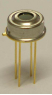
\includegraphics{analisis/imagenes/sensor_temperatura}
	\textbf{\caption{\small{Sensor de temperatura MLX9614 \cite{cuarentaycinco}.}}}
	\label{fig:sensortemperatura}
\end{figure}

A continuación, explicaremos que es un termopar y cómo es que funciona, para poder entender cómo es que funciona en sensor MLX90614.
Un termopar es una unión de dos metales distintos unidos en un extremo, cuando a la unión se le presenta una temperatura distinta a la temperatura de la unión se genera un voltaje muy pequeño (efecto Seebeck) del orden de los milivolts, esté aumenta conforme la temperatura se incrementa (no es lineal), dependiendo del tipo de termopar existe una relación temperatura-voltaje. \\

Son utilizadas como sensores de temperatura, el principal inconveniente es la necesidad de compensar a cero, esto se debe a que, al tomar las lecturas en el otro extremo del termopar, se une con otro metal distinto (creando otro termopar) produciendo otro voltaje, el cual es proporcional a la temperatura del ambiente por lo que es necesario medir la temperatura en la unión donde se realiza la lectura, utilizando un sensor que obtenga la temperatura del ambiente. Las dos temperaturas de suman para crear la compensación y así obtener la temperatura real. \\

En la figura 2.4 se muestra los puntos de intersección entre los metales, los puntos en los que se obtiene diferentes temperaturas, siendo T la temperatura del objeto y Ta la temperatura del ambiente.

\begin{figure}
	\centering
	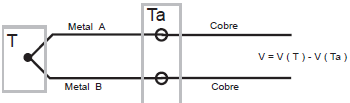
\includegraphics{analisis/imagenes/esquema_termopar}
	\textbf{\caption{\small{Esquema de un termopar (V es el voltaje total obtenido por un volmetro) \cite{cuarentayseis}.}}}
	\label{fig:esquematermopar}
\end{figure}

V(Ta) es el voltaje obtenido por la unión del metal A y el cobre \\

De tal forma que se tienen tres uniones la unión del metal A y metal B, la unión del cobre con el metal B y la unión del metal A con el cobre. Teniendo la siguiente ecuación. \\

\begin{equation}
	V_{Total} \quad = \quad V_{AB(T)} \quad - \quad V_{CuA(Ta) \quad - \quad V_{CuB(Ta)}}
\end{equation}

\begin{equation}
	V_{Total} \quad = \quad V_{AB(T)} \quad - \quad[V_{CuA(Ta) \quad - \quad V_{CuB(Ta)}}]
\end{equation}

\begin{equation}
	V_{Total} \quad = \quad V_{AB(T)} \quad - \quad V_{AB(Ta)}
\end{equation}

\begin{equation}
V_{AB(T)} \quad = \quad V_{Total} \quad - \quad V_{AB(Ta)}
\end{equation}

Posteriormente una vez que se tiene esta ecuación se busca en la tabla del termopar el voltaje $V_{AB(Ta)}$ de acuerdo a la temperatura ambiente, obteniendo el voltaje $V_{AB(T)}$ se puede saber la temperatura de la unión AB, buscando en la tabla del termopar AB, que temperatura corresponde al voltaje $V_{AB(T)}$. \\

Una vez explicado el funcionamiento de un termopar podremos entender ¿Cómo es que mide la temperatura el sensor MLX90614? El sensor MLX90614 tiene internamente dos sensores para medir la temperatura, estos sensores están conectados por medio de un termopar, la primera unión es con el sensor infrarrojo (la membrana) y la segunda con un sensor que mide la temperatura del ambiente, para posteriormente calcular la compensación del termopar y calcular la temperatura del infrarrojo \cite{cuarentayseis}. \\

La señal emitida por el termopar responde a la siguiente ecuación:

\begin{equation}
V_{Ir(Ta,To)} \quad = \quad A \quad \ast \quad (To^4 \quad - \quad Ta^4)
\end{equation}

Donde: \\

\begin{itemize}
	\item $V_{Ir(Ta,To)}$ es el voltaje de respuesta del termopar.
	\item $A$ es la sensibilidad total del infrarrojo.
	\item $To$ es la temperatura obtenida por el infrarrojo.
	\item $Ta$ es la temperatura del ambiente.
\end{itemize}

El principio de los sensores infrarrojos es la radiación infrarroja, está es la parte de la luz solar que se descompone al reflejar la luz solar a través de un prisma, la cual pose energía, teniendo relación con el espectro electromagnético. \\

La energía desprendida por la radiación del campo electromagnético se puede medir mediante una relación con las curvas emitidas por un cuerpo oscuro o negro (emisividad), mientras que los objetos con una temperatura por encima del cero absoluto irradian energía \cite{cuarentaysiete}.

\begin{figure}
	\centering
	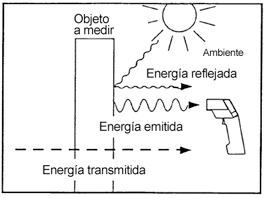
\includegraphics{analisis/imagenes/factor}
	\textbf{\caption{\small{Factor de emisión \cite{cuarentaysiete}.}}}
	\label{fig:factor}
\end{figure}

La cantidad de energía crece de manera proporcional a la cuarta potencia de la temperatura, es por ello que en la ecuación 2.20 las temperaturas $(To^4 \quad - \quad Ta^4)$, en cuanto a A es un factor de emisión que se obtuvo de la relación de las radiaciones que emite un cuerpo gris y un cuerpo negro a igual que la temperatura, estos cuerpos tienen el mismo factor de emisión  en todas las longitudes de onda, por el contrario un cuerpo diferente del gris y el negro cambia su factor de emisión con respecto a la longitud de onda. \\

La temperatura del sensor es necesaria para medir la temperatura del chip, una vez que mide la temperatura del objeto y el ambiente, se calcula la temperatura del chip, los cálculos se realizan por el DPS (Procesador de señal digital) produciendo salidas digitales lineales proporcionales a las temperaturas medidas. \\

Temperatura ambiente \\

El sensor calcula la temperatura mediante termopares y sensores de temperatura internos, todas las condiciones de los sensores y los datos procesados se manejan dentro del chip, mientras que las lecturas de la temperatura del sensor se encuentran en la memoria de acceso aleatorio (RAM) \cite{cuarentaycinco}. \\

La resolución de la temperatura calculada es de 0.02$^{\circ}$C debido a que el convertidor analógico digital (ADC) es de 17 bits, cada bit representa 0.02$^{\circ}$C, el sensor esta calibrado de fábrica con un rango de -40$^{\circ}$C a +125$^{\circ}$C, el valor digital de la temperatura ambiente se encuentra en la RAM en la celda 0x06. \\

Los valores de las temperaturas se encuentran en un formato hexadecimal, la fórmula para obtener la temperatura ambiente en grados $^{\circ}$K es la siguiente:

\begin{equation}
	Ta \quad = \quad {(Valor \quad del \quad registro \quad 0\times06)}_{10} \quad \ast \quad 0\ldotp02
\end{equation}

\begin{itemize}
	\item $Ta$ es el valor de la temperatura ambiente en grados Kelvin.
	\item Es el valor del registro después de convertir de hexadecimal a decimal.
	\item 0.02 es el valor de cada bit.
\end{itemize}

Ejemplos: \\

Tenemos que el valor de la temperatura es 0x2DE4 y se desea saber la temperatura en grados Kelvin como Celsius. \\

\begin{itemize}
	\item El primer pasó el convertir de hexadecimal a decimal el valor del registro.
\end{itemize}

Para convertir de hexadecimal a decimal se utiliza la base 16 y la base 10, multiplicamos cada dígito con el valor de la potencia base dieciséis que le corresponde, siendo el menos significativo el dígito de la derecha. \\

\begin{equation}
Valor \quad digital \quad = \quad 4\ast16^0 \quad + \quad 14\ast16^1 \quad + \quad 13\ast16^2 \quad + \quad 2\ast16^2 
\end{equation}

\begin{equation}
Valor \quad digital \quad = \quad 4 \quad + \quad 224 \quad + \quad 3328 \quad + \quad 8192 
\end{equation}

\begin{equation}
Valor \quad digital \quad = \quad {11748}_{10}  
\end{equation}

El segundo paso es multiplicar la resolución obtenida por el valor digital, obteniendo la temperatura en grados Kelvin, para pasarlos a Celsius se resta 273. \\

\begin{equation}
Ta \quad = \quad 11748 \quad \ast \quad 0\ldotp02
\end{equation}

\begin{equation}
Ta \quad = \quad 234\ldotp96^{\circ}K
\end{equation}

\begin{equation}
Ta \quad = \quad 234\ldotp96 \quad - \quad 273
\end{equation}

\begin{equation}
Ta \quad = \quad - 38\ldotp04^{\circ}C
\end{equation}

El valor mínimo de medición de la temperatura del ambiente es -38.2$^{\circ}$C y el valor máximo medido es 125$^{\circ}$C. \\
 
Temperatura Objeto \\

La temperatura del objeto se encuentra en la celda 0x07, se calcula de la misma manera que la del ambiente, el bit más significativo indica un error, al medir una temperatura que sobre pase los 382.19$^{\circ}$C o en su valor hexadecimal 0x7FFF. \\

Para obtener las mediciones de temperatura, el sensor realiza cálculos, y el resultado lo obtiene lineal, estos pasos se realizan en el núcleo del sensor (en el chip), se ejecuta un programa de la memoria de solo lectura (ROM) antes de encender o de resetear, el chip inicia con los datos de calibración, durante esta fase se selecciona el número de sensor infrarrojo que se utilizará y se decide el rango de temperatura que tendrá en sensor, las rutinas de medición, compensación y la muestra de la  temperatura lineal se corren dentro del término bucle \cite{cuarentaycinco}. \\

El sensor de temperatura utiliza los siguientes filtros para acondicionar las lecturas de temperatura: \\

Filtro Pasa-banda \\

Un filtro pasa-banda permite pasar las frecuencias que están situadas en una determinada banda de frecuencia, es decir entre dos determinadas frecuencias y rechaza las frecuencias fuera de esa banda. \\

Filtros digitales \\

Un filtro digital se puede definir como un proceso computacional o algoritmo mediante el cual una señal digital es transformada en una segunda secuencia de muestras. \\

Respuesta impulsional \\

Es la relación de un filtro a un impulso que se envía a su entrada, la respuesta impulsional caracteriza   a un filtro en el dominio temporal. El funcionamiento de un filtro digital consiste en sumar una señal de entrada a su salida o viceversa. \\

Filtros digital IR y IIR \\

El filtro IR (Respuesta impulsional finita) retarda ligeramente una copia de la señal de entrada (uno o varios periodos) y la suma a la señal de respuesta del filtro \cite{cuarentayocho}. \\ 

\begin{figure}[h]
	\centering
	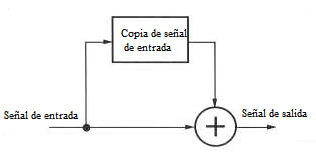
\includegraphics{analisis/imagenes/principio_filtro}
	\textbf{\caption{\small{Principio filtro FIR \cite{cuarentayocho}.}}}
	\label{fig:principiofiltro}
\end{figure}

El filtro digital IIR (Respuesta impulsional infinita) procesa una señal de entrada, la señal obtenida se combina con la de entrada.

\begin{figure}
	\centering
	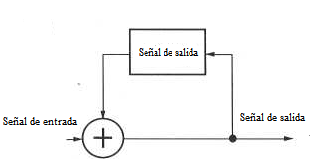
\includegraphics{analisis/imagenes/filtro_iir}
	\textbf{\caption{\small{Principio filtro IIR \cite{cuarentayocho}.}}}
	\label{fig:filtroiir}
\end{figure}

Los filtros se pueden describir mediante ecuaciones que relacionan la señal de entrada con una señal de salida en el domino digital. De manera que la salida del filtro se especifica como un resultado de sumas, restas y multiplicaciones de muestras de entradas actuales y anteriores. \\

Ecuación de los filtros digitales FIR \\

Se puede definir como la combinación lineal de muestras de la entrada presente o pasadas, se expresa de la siguiente forma:

\begin{equation}
	y[n] \quad = \quad a0 \cdot x[n] \quad + \quad a1 \cdot x[n - 1] \quad + \quad a2 \cdot x[n - 2] \quad + \ldots + \quad aN \cdot x[n - N]
\end{equation}

Esta ecuación expresa que la muestra actual de la salida $y[n]$ es igual a la suma de las muestras de la entrada actual $x[n]$ multiplicada por el factor $a0$ y de la muestra anterior $x[n – 1]$ multiplicando por el factor $a1$, y de todas las muestras anteriores hasta el instante $[n - N]$ multiplicado por su correspondiente factor. Donde los factores modifican las características de la señal \cite{cuarentayocho}. \\

Señal digital: \\

\begin{equation}
	x \quad = \quad \{1,0,0,0,0,0,0,\ldots\}
\end{equation}

Señal de salida: \\

\begin{equation}
x \quad = \quad \{a0,a1,a2,a3,\ldots,aN,0,0,0,\ldots\}
\end{equation}

Ecuación de filtro digital IIR \\

Los filtros IIR se distinguen de los filtros FIR por la presencia de una recursividad, la señal de salida del filtro retroalimenta el filtro, esté método permite implementar filtros con respuesta más compleja y con menos datos, al retroalimentar la entrada la respuesta impulsional tiene una duración potencial infinita. \\

\begin{equation*}
	\begin{split}
	y[n] \quad = \quad a0 \cdot x[n] \quad + \quad a1 \cdot x[n - 1] \quad + \quad a2 \cdot x[n - 2] \quad + \ldots + \quad \\ aN \cdot x[n - N] \quad + \quad - \quad b1 \cdot y[n-1] \quad - \quad b2 \cdot y[n-2] \quad - \quad \\ b3 \cdot y[n-3]  \quad \ldots \quad - \quad bM \cdot y[n-M]
	\end{split}		
\end{equation*}

Esta ecuación expresa que la salida es función de N+1 muestras de la entrada (actuales y N anteriores), así como de M muestras anteriores de salida. \\

Diferencia entre los filtros digitales \\

Los filtros FIR ofrecen en general una respuesta de fase más lineal y no entran jamás en oscilación, pero requieren de un gran número de muestras haciéndolos más caros computacionalmente, mientras que los filtros IIR son muy eficaces y pueden proporcionar pendientes de corte muy pronunciadas, pero tienden a entrar en resonancia\cite{cuarentayocho}. \\

Los procesos que se realizan en el sensor se dividen en 3 partes: \\

Desviación del infrarrojo \\

\begin{itemize}
	\item Se mide la desviación con la FIR, fijando la longitud de la respuesta del filtro.
	\item Agrega al filtrado la IIR fijando su longitud, el resultado es almacenado dentro de la RAM en la variable (registro) $IR_{os}$.
	\item Se obtiene otra medida con FIR del filtro, fijando la longitud de la respuesta.
	\item Compensación de la desviación.
	\item Se agrega un proceso adicional programando la longitud IIR, el resultado se almacena dentro de la RAM en $IR_G$.
	\item Se calcula la compensación obtenida, el resultado se almacena dentro de la RAM en $K_G$.
\end{itemize}

Temperatura del Objeto \\

Estos son los procesos que realizan para obtener la temperatura del objeto, el sensor MLX90614 tiene dos sensores infrarrojos internos. \\

\begin{itemize}
	\item Medición del sensor infrarrojo se programa la longitud FIR del filtro.
	\item Compensación de la desviación.
	\item Gana compensación.
	\item Se filtra, programando la longitud IIR del filtro, se almacena el resultado dentro de la RAM en la dirección 0x04 en $IR1_D$.
	\item El cálculo de la temperatura del objeto, se almacena en la dirección 0x07 en $T_{02}$.
	
\end{itemize}

El mismo procedimiento se realiza con el segundo sensor infrarrojo \cite{cuarentaycinco}.


%	   \newpage\section{An{á}lisis sensor de Pulso Card{í}aco}

Para comprender mejor el concepto de frecuencia cardíaca, empezaremos por precisar su definición posteriormente daremos paso a explicar las causas que afectan y los diferentes métodos de medición. Sin embargo, también es importante mencionar que a medida que se envejece, el deterioro fisiológico normal y la presencia de enfermedades, disminuye progresivamente la capacidad funcional. \\

La frecuencia cardíaca (FC), se define como el número de contracciones ventriculares efectuadas por el corazón, medida generalmente en latidos por minuto $(lat \bullet min^{-1})$ o pulsaciones por minuto (ppm), de tal forma que el pulso puede ser palpable en cualquier arteria \cite{cincuentayuno}. \\

El pulso es uno de los parámetros que representa la expresión periférica de la actividad del corazón. En el adulto, la frecuencia cardíaca (pulso) normal oscila entre 60 y 100 por minuto, menos de 60 se considera bradicardia la cual es extrema si el valor es inferior a 30 por minuto, más de 100 pulsaciones se considera taquicardia y es severa si sobrepasa los 170 por minuto, la severidad está determinada porque las cifras que sobrepasan estos rangos, casi siempre se asocian a síntomas de bajo gasto cardíaco (hipotensión, mareos, síncope, etc.) \cite{cincuentaydos}. \\

En las tablas 2.35, 2.36 y 2.37, se muestran los valores normales de la frecuencia cardíaca en reposo clasificados por edades y sexo.

\begin{table}
	\begin{tabular}{|p{4cm}|p{4cm}|p{4cm}|}
		\hline 
		\centering Clasificación & \centering Mujeres & \centering Hombres \\ 
		\tabularnewline
		\hline 
		Excelente & \centering $\leq$53 & \centering $\leq$56 \\ 
		\tabularnewline
		\hline 
		Bueno & \centering $60-64$ & \centering $64-57$ \\ 
		\tabularnewline
		\hline 
		Promedio & \centering $65-61$ & \centering $71-65$ \\  
		\tabularnewline
		\hline 
		Pobre & \centering $75-66$ & \centering $79-72$ \\ 
		\tabularnewline
		\hline 
		Muy Pobre & \centering $\geq$76 & \centering$\geq$80 \\ 
		\tabularnewline
		\hline 
	\end{tabular} 
	\textbf{\caption{\small{\textbf{Escala de clasificación para la frecuencia cardíaca en reposo de mujeres y hombres (latidos por minuto) \cite{cincuentaytres}}}}}
\end{table}

\newpage
\subsection{Etapas de una caída}



\end{document}
%%%%%%%%%%%%%%%%%%%%%%%%%%%%%%%%%%%%%%%
%%%%%%%    FIN DEL DOCUMENTO    %%%%%%%
%%%%%%%%%%%%%%%%%%%%%%%%%%%%%%%%%%%%%%%
